\documentclass[12pt,a4paper,openright,twoside]{book}
\usepackage[utf8]{inputenc}
\usepackage{disi-thesis}
\usepackage{code-lstlistings}
\usepackage{notes}
\usepackage{shortcuts}
\usepackage{acronym}
\usepackage{svg}
\usepackage{multirow}
\usepackage{subcaption}

\school{\unibo}
\programme{Corso di Laurea Magistrale in Ingegneria e Scienze Informatiche}
\title{Type-Safe Complex Specifications in Kotlin: a DSL to Configure the Alchemist Simulator}
\author{Marco Frattarola}
\date{\today}
\subject{Software Process Engineering}
\supervisor{Prof. Gianluca Aguzzi}
\cosupervisor{Dott. Danilo Pianini}
\morecosupervisor{}
\session{I}
\academicyear{2024-2025}

% Definition of acronyms
\acrodef{IoT}{Internet of Thing}
\acrodef{vm}[VM]{Virtual Machine}


\mainlinespacing{1.241} % line spacing in mainmatter, comment to default (1)

\begin{document}

\frontmatter\frontispiece

\begin{abstract}	
Max 2000 characters, strict.
\end{abstract}

\begin{dedication} % this is optional
Optional. Max a few lines.
\end{dedication}

%----------------------------------------------------------------------------------------
\tableofcontents   
\listoffigures     % (optional) comment if empty
\lstlistoflistings % (optional) comment if empty
%----------------------------------------------------------------------------------------

\mainmatter

%----------------------------------------------------------------------------------------
\chapter{Introduction}
\label{chap:introduction}
%----------------------------------------------------------------------------------------

Simulating complex systems is a key part of modern research and engineering.
These systems are made up of many parts that interact with each other, creating behaviors that are hard to predict 
just by looking at the individual pieces.
To study things like how biological networks work or how a swarm of robots moves,
powerful simulation tools that can handle space, time, and randomness are required.

Alchemist is one such tool, designed to model these kinds of distributed systems.
But as simulations get more complicated, setting them up becomes a real challenge.
Right now, users have to write configuration files in YAML\footnote{\url{https://yaml.org/}}.
While YAML is easy to read in simple scenarios, it becomes hard to read and maintain in more complex scenarios. 
It also does not help to check if the configuration is actually correct 
until the simulation is executed.
This leads to frustration, errors, and wasted time.

This thesis proposes a better way to configure Alchemist simulations.
Rather than relying on static text files, a Kotlin-based Domain-Specific Language (DSL)~\cite{fowler2010domain} has been created. 
This enables users to author their configurations in a code-like manner, offering numerous advantages.
Checks are performed while typing, suggestions are provided by the Integrated Development Environment (IDE), 
and the chance of making mistakes is significantly reduced.
The goal is to make the process of setting up a simulation smoother and more reliable, enabling researchers to focus on their experiments 
rather than fighting with configuration files.

This thesis is organized as follows. 
\begin{itemize}

    \item Section~\ref{sec:context-motivation} details the context and motivation behind this project.
    \item Section~\ref{sec:background} provides background information about the Alchemist simulator and the 
    concept of Domain-Specific Languages.
    \item Chapter~\ref{chap:analysis} analyzes the requirements and constraints for developing the DSL,
    examining the limitations of the current YAML approach and establishing the domain model. 
    \item Chapter~\ref{chap:design} presents the design of the DSL, including its architecture and key design decisions. 
    \item Chapter~\ref{chap:implementation} describes the implementation details and challenges encountered during development. 
    \item Chapter~\ref{chap:evaluation} presents the evaluation of the DSL, detailing the methods and results of the assessments performed.
    \item Chapter~\ref{chap:conclusion} summarizes the contributions and discusses future work.
\end{itemize}

\newpage
\section{Context and Motivation}
\label{sec:context-motivation}
\subsection{Configuring Complex Systems}

Configuration constitutes a fundamental mechanism through
which users specify the structure, behavior, and parameters
of complex systems without modifying the underlying implementation. 
In the context of computational systems, configuration encompasses 
the specification of runtime characteristics, architectural topology,
behavioral policies, and experimental parameters that govern system
execution. Rather than encoding these aspects directly into program 
logic, configurations externalize them into separate artifacts that 
can be modified, versioned, and reused independently of the core 
codebase. This separation of concerns enables a single implementation 
to serve diverse use cases through different configurations.
To facilitate configuration authoring, many systems develop specialized 
Domain-Specific Languages (DSLs) tailored to their configuration needs. 
These DSLs provide syntax and abstractions that align with the domain concepts 
of the target system, making configurations more intuitive and less error-prone 
than generic data formats. Prominent examples include Docker's Dockerfile syntax\footnote{\url{https://docs.docker.com/reference/dockerfile/}}
for container image construction, Kubernetes manifests\footnote{\url{https://kubernetes.io/docs/concepts/workloads/controllers/deployment/}}
for orchestrating containerized 
applications, Spring Boot's\footnote{\url{https://docs.spring.io/spring-boot/index.html}} application properties and YAML configurations for 
dependency injection and application setup, Gradle's\footnote{\url{https://gradle.org/}} build configuration DSL 
for defining build scripts and dependencies. For example, in a simulation framework 
like Alchemist a simulation can be defined by creating a configuration 
file that specifies all the needed parameters such as the initial state and the 
behavior of its components. This configuration file can then be used to create a 
simulation instance that can be run.

    
\newpage
\subsubsection{Imperative and Declarative Configuration Paradigms}

Configuration management systems can be classified according to 
two distinct paradigms that fundamentally differ in their approach 
to system specification and manipulation: 
\begin{itemize}
    \item \textbf{Imperative paradigm}
    \item \textbf{Declarative paradigm}
\end{itemize}

This distinction, 
 rooted in the dichotomy between procedural and declarative 
 programming models, has profound implications for how 
 systems are configured, maintained, and reasoned about.

The \textit{imperative configuration} paradigm focuses on specifying \textbf{how} 
a system should reach its desired state through explicit sequences of 
commands and operations. An imperative configuration defines 
the procedural \textbf{steps} required to transform the system from its 
current state to the \textit{target state}. Each command represents an 
action that modifies system state, and the execution order is 
critical to achieve the intended outcome. Shell scripts and traditional system 
administration procedures exemplify this approach.
Another example of an imperative configuration is the \textit{Dockerfile} configuration file:
Docker is an open platform for developing, shipping, and running applications.
A \textit{Dockerfile} is the Docker's imperative configuration 
format for building container images. 
It is a text file containing instructions for building source code. 

\begin{minted}[fontsize=\footnotesize, linenos]{dockerfile}
FROM ubuntu:22.04
# install app dependencies
RUN apt-get update && apt-get install -y python3 python3-pip
RUN pip install flask==3.0.*
# install app
COPY hello.py /
# final configuration
ENV FLASK_APP=hello
EXPOSE 8000
CMD ["flask", "run", "--host", "0.0.0.0", "--port", "8000"]
\end{minted}
\captionof{lstlisting}
{Example of a Dockerfile configuration}

In this example, each \texttt{RUN}, \texttt{COPY}, and \texttt{CMD} instruction represents
 a step that modifies the container image state, 
 and the sequence must be carefully ordered 
 (e.g., installing packages before executing files that depend on them). 
 Docker then builds images by reading the instructions from a Dockerfile.

In contrast, the declarative configuration paradigm focuses 
on specifying \textbf{what} the desired system state should be,
abstracting away the procedural details of how that state is achieved. 
A declarative configuration describes the target state as a set
of constraints, properties, and resource specifications, 
delegating to the configuration management 
system the responsibility of determining and executing the
necessary operations to realize that state. 
The system automatically computes the necessary
set of changes required to achieve the desired state. 
Tools such as Docker Compose, Puppet\footnote{\url{https://help.puppet.com}}, 
Terraform\footnote{\url{https://developer.hashicorp.com/terraform/language}} and Kubernetes manifests 
exemplify this paradigm. 
Docker Compose, for example, allows developers to declare 
the desired state of multi-container applications using a YAML file:
\begin{minted}[fontsize=\footnotesize, linenos]{yaml}
services:
  web:
    build: .
    ports:
      - "8000:5000"
  redis:
    image: "redis:alpine"
\end{minted}
\captionof{lstlisting}
{Example of a Docker Compose configuration}

The declarative paradigm offers several advantages that have driven its
adoption across modern infrastructure management. 
\begin{enumerate}
    \item Declarative configurations are
    inherently more readable and maintainable, as they document the intended system state
    without obscuring it with implementation details.
    \item They are idempotent by design:
    applying the same configuration multiple times produces the same result, eliminating concerns
    about partial execution or repeated application.
    \item They facilitate reasoning about system properties through formal verification
     and constraint validation before deployment.
    \item They support more robust error handling, as the system
    can detect when the desired state cannot be achieved and report specific discrepancies.
\end{enumerate}

\subsubsection{Application Domains}

Declarative configuration systems have proliferated across diverse domains of software infrastructure, 
each addressing specific challenges. Understanding these application domains and their
 representative technologies provides 
context for the subsequent discussion of configuration challenges and the motivation
for type-safe configuration approaches proposed in this thesis.
Some application domains and representative systems are:
\begin{itemize}

\item \textbf{Infrastructure Configuration Management}:
Puppet pioneered the declarative configuration management paradigm for
physical and virtual server infrastructure.
Its resource abstraction model allows administrators to declare desired states for files,
packages, services, users, and other system entities.
Chef\footnote{\url{https://docs.chef.io/}} followed a similar philosophy while embedding configuration logic within a
Ruby domain-specific language, providing both declarative resource declarations and 
imperative programming constructs. 
These tools revolutionized system administration by replacing ad-hoc shell
scripts with version-controlled, testable configuration artifacts.

\item \textbf{Cloud Infrastructure Provisioning}:
Terraform extended declarative configuration to cloud resource provisioning, 
allowing operators to declare entire cloud environments, including compute instances, 
networks, load balancers, databases, and access policies, using a unified configuration language. 

\item \textbf{Container Orchestration}:
Kubernetes represents perhaps the purest expression of declarative configuration in modern infrastructure.
 The Kubernetes API defines a comprehensive schema of resource types such as 
 Pods, Services, Deployments, ConfigMaps, Secrets, and dozens of others,
 Users express desired states through YAML or JSON manifests, and Kubernetes controllers
  continuously reconcile actual cluster state with declared specifications.
\item \textbf{Build Automation}:
Build automation tools like Gradle provide hybrid models that combine
declarative DSLs with imperative logic when needed.

\item \textbf{Complex Systems Configuration}:
Scientific simulation frameworks like Alchemist employ 
declarative configuration files to specify complex experimental scenarios. 
Other simulation platforms, such as Eclipse MOSAIC\footnote{\url{https://eclipse.dev/mosaic/docs/}} for connected mobility simulations
and AWS SimSpace Weaver\footnote{\url{http://archive.today/BUt4k}} for large-scale spatial simulations, similarly utilize
declarative configuration files (JSON and YAML respectively) to define
simulation parameters and system structures. This approach enables researchers 
and developers to express sophisticated configurations 
without imperative programming, facilitating reproducibility 
and systematic parameter exploration.
\end{itemize}

These systems, while addressing distinct domains, share common architectural patterns:
\begin{itemize}
    \item{\textbf{Resource schema}}: defines the universe of entities that the configuration system can manage, 
    specifying the types of resources, their properties, validation rules, and semantic constraints. It 
    is the abstract model of the configuration system.
    \item{\textbf{Concrete syntax}}: provides a human-readable, version-controllable format for expressing configurations,
    supporting necessary abstraction, parameterization, and composition. Some systems, like Gradle and Terraform, 
    provide domain-specific languages with built-in
    abstraction primitives such as modules, variables, and iteration constructs. Others, like Kubernetes,
     define a pure data format (JSON/YAML). Different concrete syntaxes can target the same underlying resource schema.
    \item{\textbf{Configuration management engine}}: it is responsible for determining a valid sequence 
    of operations to achieve the desired state (respecting dependencies and constraints), 
    and execute those operations while handling errors and partial failures. 
\end{itemize}


\subsection{Challenges and Limitations}

Despite the architectural sophistication of declarative configuration systems,
 the concrete syntax layer has converged on a remarkably narrow set of data serialization formats. 
 XML (Extensible Markup Language), JSON (JavaScript Object Notation), 
 YAML (YAML Ain't Markup Language) have emerged as the most used data formats for expressing configuration artifacts 
 across different domains of modern software infrastructure. 
 This convergence reflects their perceived advantages: 
 human readability, widespread tool support, and interoperability with programming language data structures. 
 However, these formats have fundamental limitations that become increasingly problematic as configuration 
 complexity grows.

\subsubsection{Lack of Type Safety}

XML, JSON and YAML are fundamentally \textit{untyped} data formats. 
They represent data structures (objects, arrays, strings, numbers, booleans, and null values) without any 
mechanism for expressing type constraints, 
required fields, or value ranges. 
Type information exists only implicitly through runtime validation performed by the consuming application, 
which must parse the configuration and verify that values conform to expected types and constraints. 
This validation occurs entirely at runtime, meaning configuration errors surface only when the system attempts 
to load or execute the configuration,
 potentially after significant development effort has been invested.

Beyond the absence of type constraints, XML, JSON and YAML are fundamentally limited to primitive data
 types supported by 
the serialization format itself. 
These formats natively support only basic scalar types along with composite structures (objects and arrays) 
composed of these primitives.
This limitation becomes particularly problematic when configuration systems need to express domain-specific 
concepts that
 map to programming language classes, interfaces, or complex object types. 

Consider simulation frameworks like Alchemist, where configurations must specify classes that
 will be instantiated at runtime to
 represent domain entities. The YAML configuration expresses these class specifications as string literals:

\begin{minted}[fontsize=\footnotesize, linenos]{yaml}
incarnation: protelis
environment:
  type: Continuous2DEnvironment

network-model:
  type: ConnectWithinDistance
  parameters: [6]

deployments:
  type: Rectangle
  parameters: [1, 0, 0, 100, 100]
\end{minted}
\captionof{lstlisting}{Example of an Alchemist YAML configuration with class loading}

Here, class names such as \texttt{Continuous2DEnvironment}, 
\texttt{ConnectWithinDistance} and
\texttt{Rectangle} are specified as plain strings. 
The application must use reflection or factory patterns to resolve these string class 
names to actual Java or Kotlin classes at runtime, 
instantiate them with the provided parameters,
 and verify that the constructor signatures match. 
 This approach introduces several critical problems such as:

\begin{itemize}
    \item \textbf{No compile-time verification}: The class name is merely a string literal, 
    so there is no way to verify at configuration authoring time that the specified class exists, 
    is accessible, or implements the expected interface.
    \item \textbf{No constructor parameter validation}: The parameters array must match the constructor signature, 
    but this compatibility cannot be checked statically. 
    A mismatch between parameter count, types, or order is discovered only when instantiation fails at runtime.
    \item \textbf{No type inference or IDE support}: Since class names are strings, Integrated Development Environments (IDEs)
     cannot provide autocomplete suggestions,
     type-aware parameter hints, or navigation to class definitions.
   \item \textbf{Refactoring}: Renaming a class in the codebase requires manually updating all string references in configuration files,
     with no tooling support to ensure completeness.
\end{itemize}

This pattern of specifying class names as strings for runtime instantiation is not unique to Alchemist. 
Many frameworks employ similar approaches across different domains. 
The Spring Framework , for instance, allows developers to define beans and their dependencies in XML 
configuration files\footnote{\url{http://archive.today/p3ANv}},
 where class names are specified as strings:

\begin{minted}[fontsize=\footnotesize, linenos]{xml}
<bean id="item1" class="org.baeldung.store.ItemImpl1" /> 
<bean id="store" class="org.baeldung.store.Store"> 
    <constructor-arg type="ItemImpl1" index="0" name="item" ref="item1" /> 
</bean>
\end{minted}
\captionof{lstlisting}{Example of a Spring Framework XML configuration}

Spring's dependency injection container resolves these string class names at runtime, 
instantiating the classes and wiring dependencies. 
Moreover, when configurations involve nested object construction, 
where one class requires another class as a parameter, 
the problem compounds. 
Consider an Alchemist configuration specifying
 a time distribution that itself requires other time distribution objects:

\begin{minted}[fontsize=\footnotesize, linenos]{yaml}
time-distribution:
  type: JaktaTimeDistribution
  parameters:
    sense:
      type: WeibullTime
      parameters: [1, 1]
    deliberate:
      type: DiracComb
      parameters: 0.1
    act:
      type: ExponentialTime
      parameters: 1
\end{minted}
\captionof{lstlisting}{Example of an Alchemist YAML configuration with nested objects}

The absence of compile-time type checking means that refactoring configurations is inherently risky.
Renaming a service, changing a parameter structure, or modifying nested configurations requires manual verification 
that all references have been updated correctly. 
In complex configurations spanning multiple files or involving hundreds of interdependent components, 
this manual process is error-prone and time-consuming.
Type mismatches, missing required fields, and inconsistent parameter combinations are discovered only through runtime failures, 
forcing users to debug through opaque error messages and stack traces rather than receiving immediate, 
actionable feedback during configuration authoring.

\subsubsection{Limited Developer Experience}

The absence of type information significantly restricts the functionality of Integrated Development Environments (IDEs) and text editors. 
When explicit schemas or type specifications are missing, 
IDEs are unable to offer useful autocomplete features, embedded documentation, or immediate error identification. 
Users must depend on separate documentation to learn about available configuration parameters, expected data types, and applicable restrictions. 
This lack of IDE assistance steepens the learning process for newcomers and diminishes efficiency even among seasoned users.

Validation mechanisms based on schemas are available for JSON, YAML, and XML formats, providing a certain level of 
structural checking and enhanced IDE functionality. JSON Schema\footnote{\url{https://json-schema.org/specification}}
provides a uniform method for specifying the anticipated structure of JSON files, whereas XML Schema Definition (XSD)\footnote{\url{http://archive.today/G557h}} 
delivers comparable features for XML. YAML configurations can utilize JSON Schema or YAML-tailored schema specifications to verify document organization,
 mandatory fields, and fundamental type requirements.

Nevertheless, schema-based validation offers only incomplete remedies to the core limitations of untyped configuration formats. 
Although schemas can check syntax—confirming that mandatory fields exist, that values match expected basic types, and that document 
structure aligns with a specified template, they deliver restricted support for business logic and semantic verification.

In the case of a system that supports class loading, including Alchemist, a schema author 
could enumerate all possible class names that may appear in a \texttt{type} field, 
allowing the schema to validate that the string represents one of the known classes. Similarly, 
a schema could specify the expected parameter count and types for each enumerated class, enabling validation of constructor compatibility. 
However, this approach requires the schema author to maintain a complete, exhaustive list of all classes that may be instantiated, 
along with their constructor signatures. 
For closed systems with a fixed set of types, this is feasible and can provide meaningful validation.

The fundamental challenge arises in \textit{extensible} software systems like Alchemist, 
where the set of valid class types is open-ended and cannot be fully captured in a static schema definition. 
A schema author attempting to enumerate all possible classes would face a challenging task: 
the schema would need to be updated every time a new plugin or extension is developed, or use an 
automated tool to generate it. 

Moreover, schemas cannot validate semantic relationships that require understanding the runtime behavior of classes. 
For instance, schemas cannot ensure that YAML anchor references resolve correctly, 
that variable dependencies form a valid acyclic graph, or that mathematical expressions in configuration values
 are well-formed and type-safe. 
These validations require understanding the semantics of the configuration language and the relationships 
between configuration elements, 
which goes beyond what structural schemas can express.

These schemas are typically external to the configuration file itself and 
require explicit configuration of IDE plugins or validation tools. 
The developer experience contrasts sharply with that of statically-typed programming languages, 
where IDEs provide comprehensive autocomplete, type checking, refactoring support, 
and inline documentation based on the language's type system.

\subsubsection{Readability and Maintainability Challenges}

As configuration complexity increases, JSON and YAML files become increasingly difficult to read, 
understand, and maintain.
The hierarchical structure of these formats, while useful for simple configurations, 
becomes unwieldy when dealing with systems
 involving dozens of components, deeply nested structures, or complex interdependencies.
 It is not uncommon to see configurations with hundreds of lines of code,
  making it difficult to understand and maintain.

Another issue of untyped configuration formats is the lack of mechanisms to reduce 
duplication within a single file. Some formats do provide limited mechanisms 
to reduce duplication such as YAML that supports anchors and aliases\footnote{\url{http://archive.today/bcJbb}}
that allow defining 
a value once and referencing it multiple times within the same document. 
However, these mechanisms are fundamentally limited: they operate only within a single file, 
cannot reference external files, and provide no type safety or compile-time validation of references. 
JSON provides no built-in mechanism for reuse whatsoever, requiring complete duplication of common patterns.

More critically, none of these formats provide standardized mechanisms for dividing configurations 
across multiple files and reusing components across different configuration files, 
as one would expect in a programming language where classes and functions can be defined 
in separate modules 
and imported where needed. While XML provides standardized mechanisms for including external files 
such as \textit{XInclude}\footnote{\url{https://www.w3.org/TR/xinclude-11/}}, YAML and JSON have no such standard capabilities. 
This limitation forces users of the configuration system to either maintain monolithic configuration files 
or rely on external preprocessing tools that merge files before parsing, 
neither of which provides the type safety, IDE support, or refactoring capabilities 
that would be available if configurations could be structured as reusable, 
type-checked modules similar to programming language components. Complex applications, like
Alchemist, could benefit from this by being able
 to define reusable components that can be shared across different simulations.

The limitations of JSON and YAML formats become particularly pronounced when configuring complex 
scenarios such as scientific simulations and experimental configurations. 
Expressing complex scenarios in YAML results in very long files that tend to 
grow more vertically rather than horizontally (see listing~\ref{lst:examplecomplexsimulation}), where the  
semantic relationships between configuration elements are obscured by syntactic boilerplate. 

\begin{center}
    \begin{minipage}{0.48\textwidth}
    \inputminted[
      fontsize=\tiny,
      breaklines,
      firstline=1,
      lastline=59, 
      linenos
    ]{yaml}{listings/examplecomplexsimulation.yaml}
    \end{minipage}
    \hfill
    \begin{minipage}{0.48\textwidth}
    \inputminted[
      fontsize=\tiny,
      breaklines,
      firstline=60,
      lastline=119, 
      linenos
    ]{yaml}{listings/examplecomplexsimulation.yaml}
    \end{minipage}
    \captionof{lstlisting}
    {Example of a complex Alchemist simulation configuration \protect~\cite{domini2025fbfl}}
    \label{lst:examplecomplexsimulation}
\end{center}
\newpage


Parameter references must be expressed as strings, making it
impossible to verify referential integrity statically. 
Mathematical expressions and conditional logic must be encoded as strings or 
complex nested structures, losing the clarity and type safety that programming 
language constructs would provide. The lack of abstraction mechanisms
beyond simple variable substitution means that common patterns must be repeated rather 
than abstracted into reusable components.


\subsubsection{Error Handling and Runtime Validation}

As configuration systems scale to complex scenarios, the error handling and validation mechanisms 
in YAML, JSON, and XML reveal fundamental limitations that make debugging difficult and error-prone. 
Unlike statically-typed programming languages where errors are caught at compile-time with precise 
location information and clear diagnostic messages, configuration formats provide only runtime validation, 
and the error messages they produce are often ambiguous, unhelpful, or point to internal parser mechanisms 
rather than the actual configuration problem.

One of the most insidious aspects of YAML's indentation-based syntax is that a misindented line can produce 
a syntactically valid document that parses successfully, but with a completely different semantic meaning 
than intended. Consider the following Alchemist configuration:

\begin{minted}[fontsize=\footnotesize, linenos]{yaml}
incarnation: sapere
environment:
  type: Continuous2DEnvironment
  parameters: [100, 100]
network-model: {type: ConnectWithinDistance, parameters: [5]}
\end{minted}
\captionof{lstlisting}{Example of a correct Alchemist YAML configuration}

\newpage
If a single extra space is accidentally added before \texttt{network-model}, the YAML parser will interpret 
it as a nested key under \texttt{environment}:

\begin{minted}[fontsize=\footnotesize, linenos]{yaml}
incarnation: sapere
environment:
  type: Continuous2DEnvironment
  parameters: [100, 100]
  # Extra tab before this line
  network-model:  {type: ConnectWithinDistance, parameters: [5]}
\end{minted}
\captionof{lstlisting}{Example of an Alchemist YAML configuration with incorrect indentation}

This configuration is syntactically valid and will parse without error, but the \texttt{network-model} 
will be incorrectly nested under \texttt{environment} rather than being a top-level configuration key. 
In this case the application will produce two different simulation results:
\begin{itemize}
    \item The first file will produce a simulation with the specified network model (\textit{ConnectWithinDistance}).
    \item The second file will produce a simulation where the network model is ignored, and 
    the default network model is used (\textit{NoLinks}).
\end{itemize}

The user must manually inspect the file, and check indentation levels to identify the root cause,
 a time-consuming process that becomes even more difficult as configuration files 
 grow to hundreds of lines. These kinds of errors are particularly insidious because the configuration file 
 is still a valid file and the application may not always produce an error message.
The problem compounds when configurations reference values that are validated only at application runtime. 
For example, a Spring Boot beans configuration XML file might specify a class name that does not exist:

\begin{minted}[fontsize=\footnotesize, linenos]{xml}
<bean id="nonExistentBean" class="com.example.NonExistentClass">
    <property name="someProperty" value="test"/>
</bean>
\end{minted}
\captionof{lstlisting}{Example of a wrong Spring XML configuration}

The XML parser will accept this configuration as valid, since \texttt{NonExistentClass} 
is a perfectly valid string. The error will only surface when the application attempts to instantiate 
the class at runtime.
\begin{minted}[
    fontsize=\footnotesize,
    linenos
]{java}
[...]
Caused by: java.lang.ClassNotFoundException: com.example.NonExistentClass
    at java.base/jdk.internal.loader.BuiltinClassLoader.loadClass
    at java.base/jdk.internal.loader.ClassLoaders$AppClassLoader.loadClass
[...]
\end{minted}
\captionof{lstlisting}{Example of a Spring boot runtime error message}

As configuration complexity increases, with complex nested structures and interdependent 
parameters, these error handling limitations become severe productivity bottlenecks. It is not always
immediately obvious to the user to pinpoint the root cause of the error. In this case a simple mistake in the 
fully qualified name of the class will cause a \textit{ClassNotFoundException} since the application
is not able to locate the exact position of the class in the classpath.
 This makes it difficult to debug the configuration error.
Users spend significant time debugging configuration errors
 that could be caught immediately with compile-time validation, 
clear error messages, and IDE support that highlights problems as they type. The lack of early error detection 
means that configuration errors are discovered only after the system attempts to execute, potentially after 
significant computation has already occurred or after a deployment has been initiated, making the debugging 
process even more costly and frustrating.

\newpage

\subsection{The Need for a Type-Safe Configuration Language}
Recent configuration languages demonstrate that declarativity can coexist with type safety and tooling support. 
Configuration tools like CUE\footnote{\url{https://cuelang.org/docs/}} unify data, schemas, and policies inside a single constraint system, 
enabling incremental validation,
order-independent unification, and reusable templates that reduce boilerplate.
Dhall\footnote{\url{https://docs.dhall-lang.org}} delivers a total, strongly typed language whose expressions normalize 
deterministically and can be exported to YAML or JSON
without sacrificing safety guarantees\footnote{\url{https://archive.is/uNGdr}}.


These languages are not widely adopted, but they motivate the need for a type-safe configuration language,
in the sense that they show that declarativity can coexist with type safety and tooling support.
Another good example is 
Gradle, that provides a hybrid model that combines declarative DSLs with imperative logic when needed, giving the user
the best of both worlds.
In this thesis we propose a type-safe configuration language for the Alchemist simulator, using Kotlin as the implementation 
language.


The need for a type-safe configuration language is motivated by the limitations of the current YAML-based configuration system, 
as described in the previous section, and by the requirement for a more powerful configuration mechanism that can accommodate 
the extensibility of the Alchemist simulator and the complex scenarios it enables. 
Kotlin was chosen for several reasons: 
first, the language provides first-class support for building domain-specific languages through its expressive DSL builders 
and extension functions that enable creating fluent, readable configuration APIs. 
Second, Alchemist is a JVM-based framework originally implemented in Java, Kotlin, and Scala, 
which means Kotlin is already natively supported within the Alchemist ecosystem without requiring additional runtime dependencies 
or cross-language interoperability layers.
 This native integration ensures seamless compatibility with existing Alchemist codebases 
and enables direct access to the framework's APIs and domain models. 


Kotlin's static type system, combined with its DSL capabilities and IDE ecosystem, makes it possible to encode domain 
entities and relationships as first-class constructs that the compiler can verify. Type safety is therefore elevated from 
an ergonomic preference to a correctness requirement: configuration authors receive compile-time diagnostics, 
refactoring support, 
and reusable libraries that can be shared between different projects.

\section{Background}%----------------------------------------------------------------------------------------

\label{sec:background}
%----------------------------------------------------------------------------------------

This section provides the background information for this thesis work. 
We begin by introducing the Alchemist simulator, describing what it is and how it 
is used across various application domains.
Then we give a definition for the concept of Domain-Specific Language (DSL), 
and explore more in detail the usage of Kotlin to 
build Domain-Specific Languages.


\subsection{Alchemist}

Alchemist is a general-purpose simulation framework designed for modeling
 spatially-distributed systems with temporal dynamics. 
The project originated in 2010 as part of the European SAPERE\footnote{\url{https://archive.is/umlcC}} project (Self-Aware Pervasive Service Ecosystems), 
initially conceived as a chemical-oriented multi-compartment 
stochastic simulation engine capable of supporting compartment mobility 
while maintaining high performance, adopting an extended version of the 
\textit{Gibson and Bruck's Next Reaction Method}~\cite{bruck}, that is able to support 
different rules (reactions) in different compartments~\cite{alchemisttutorial}. Since its inception, 
Alchemist has evolved into a comprehensive simulation platform that 
transcends its original chemical domain, 
enabling researchers to model diverse phenomena 
ranging from biochemical networks to distributed computing systems, 
crowd dynamics, and swarm robotics.

What distinguishes Alchemist from domain-specific simulators is its extensible \textit{meta-model} architecture. 
Rather than being constrained to a single application domain, the framework 
employs a loose interpretation of its core abstractions, 
enabling different \emph{incarnations} to specialize the framework for specific domains 
while maintaining a unified simulation engine. 
This design philosophy allows Alchemist to serve as a versatile platform
 where domain experts can focus on their specific modeling needs 
without reimplementing core simulation infrastructure.

The simulation engine is incarnation-agnostic, 
while domain-specific functionality is encapsulated within incarnations that can be developed
 and extended independently.
 Alchemist simulations are configured via YAML files, 
 following a YAML specification \footnote{\url{https://alchemistsimulator.github.io/reference/yaml/index.html}}.
 The configuration system is very extensible and allows to configure the simulation in a very flexible way, 
 allowing the user to have full control over the simulation configuration.
 However, it suffers from fundamental YAML-based configuration limitations, 
 described in the previous section, that become increasingly problematic as simulation 
 complexity grows.


\subsubsection{Core Concepts and Meta-Model}

Alchemist's meta-model provides a unified abstraction
for modeling spatially-distributed systems through a chemical-inspired computational paradigm. 
The framework's core abstractions enable the simulation of diverse phenomena 
while maintaining a consistent conceptual model. 
Figure~\ref{fig:alchemist-metamodel} illustrates the relationships between the main entities of the Alchemist meta-model.

\begin{figure}[H]
    \makebox[\textwidth][c]{\includesvg[width=420pt]{figures/meta}}
    \caption{The Alchemist meta-model~\cite{alchemisttutorial}}
    \label{fig:alchemist-metamodel}
\end{figure}

The meta-model is organized around the following fundamental concepts:

\begin{itemize}
    \item \textbf{Data representation}:
    \begin{itemize}
        \item \emph{Molecules}: Identifiers for data items, analogous to variable names in imperative programming languages.
         A molecule serves as a key that uniquely identifies a piece of information within a node.
        \item \emph{Concentrations}: Values associated with particular molecules, similar to values stored in variables. 
        The terminology derives from chemistry but applies generically: 
        molecules and concentrations can represent any data type, enabling the framework to model diverse 
        domains beyond chemical systems. 
        The loose interpretation of these concepts is fundamental to Alchemist's extensibility, 
        as different incarnations can define concentration types appropriate for their specific domain.
    \end{itemize}
    
    \item \textbf{Spatial organization}:
    \begin{itemize}
        \item \emph{Nodes}: Containers that hold molecules and reactions, representing entities within the simulated system. 
        Each node maintains local state through its molecules and executes reactions that modify this state over time.
        \item \emph{Environments}: Provide spatial services essential for modeling distributed systems. 
        The environment tracks node positions, computes distances between nodes, and optionally supports node mobility. 
        Environments may be continuous, representing Euclidean spaces with real-valued coordinates, or discrete, 
        representing graphs or grids. This flexibility accommodates different spatial modeling needs,
         from continuous physical spaces to discrete network topologies.
        \item \emph{Linking rules}: Functions that determine connectivity between nodes based on the current state of 
        the environment. 
        Each linking rule maps nodes to \textit{neighborhoods}, where a neighborhood consists of a center node and a set of 
        neighboring nodes. 
        This mechanism models communication constraints and interaction patterns, 
        such as distance-limited wireless networks where nodes interact only with nearby neighbors. 
        The linking rule dynamically updates neighborhoods as nodes move or as the environment changes, 
        enabling the simulation of mobile systems with evolving connectivity patterns.
        \item \emph{Neighborhoods}: Entities composed of a center node and its set of neighboring nodes, representing the local interaction context for each node.
    \end{itemize}
    
    \item \textbf{Behavioral specification}:
    \begin{itemize}
        \item \emph{Reactions}: Define the behavior and evolution of the system. 
        Each reaction comprises three essential components:
        \begin{itemize}
            \item \emph{Conditions}: Functions that evaluate the current environment state and 
            determine whether the reaction can execute.
            If a condition does not hold, the associated reaction cannot run.
            \item \emph{Actions}: Operations that modify the environment when the reaction fires, 
            changing molecule concentrations, node positions, or other system state.
            \item \emph{Time distribution}: Determines when reactions occur based on an instantaneous rate computed 
            from static parameters and condition values. 
            This stochastic modeling approach enables reactions to occur with probabilities 
            that depend on the current system state, creating realistic temporal dynamics where reaction
             frequencies adapt to environmental conditions.
        \end{itemize}
        The reaction mechanism enables the expression of complex behaviors through composition. 
        Multiple conditions can be combined to create sophisticated reaction rules, while actions can modify multiple
         molecules simultaneously or trigger cascading effects. 
         The time distribution can model various stochastic processes, 
         from exponential distributions for memoryless events to more complex distributions that capture 
         domain-specific timing characteristics.
    \end{itemize}

As previously noted, the framework includes several built-in \textit{incarnations}, each tailored to specific application domains.
Each incarnation defines type systems for concentrations and specializes the framework for specific domains.
It provides a concrete instantiation of the Alchemist meta-model by specifying the data 
types that concentrations can assume and providing domain-specific conditions, actions, environments, 
and reactions that operate on those types. 
Some of the built-in incarnations are:
    \item \textbf{SAPERE incarnation}: The initial stable incarnation developed within the European 
    SAPERE project. 
    It introduces \emph{Live Semantic Annotation} (LSA), dynamic representations of resource state
     (sensors, services, actuators).
     In Alchemist, LSAs are implemented as tuples through \texttt{LsaMolecule}, 
    stored as node data. Their evolution follows \emph{Eco-Laws}, rewriting rules similar to chemical 
    reactions that 
    consume matching tuples and produce new ones, creating ecosystem-like behaviors\footnote{\url{https://alchemistsimulator.github.io/explanation/sapere/index.html}}.
    \item \textbf{Protelis incarnation}: Integrates the Protelis~\cite{protelis} aggregate programming language,
    enabling the simulation of distributed algorithms where computations emerge from local interactions between nodes.
    \item \textbf{Scafi incarnation}: Supports the ScaFi~\cite{scafi} framework for field-based computing, 
    providing similar capabilities for aggregate programming scenarios.
    \item \textbf{Biochemistry incarnation}: Provides detailed biochemical reaction modeling capabilities, 
    supporting reactions that occur within cells, between cells, and between cells and their environment, 
    including support for cell junctions and collisions.
\end{itemize}

This incarnation-based architecture enables a unified simulation engine 
to support multiple modeling paradigms while 
allowing researchers to extend the framework with custom incarnations for specialized domains.

\subsubsection{Application Domains}

Alchemist has been employed to simulate complex scenarios across multiple domains, 
demonstrating the framework's versatility and effectiveness. Some of them are:

\begin{itemize}
    \item \textbf{Biochemical reaction networks}: Modeling the dynamics of chemical reactions in biological systems,
     where molecules represent chemical species and reactions model biochemical processes. 
    These simulations enable researchers to understand how complex biochemical networks behave under 
    different conditions and parameter settings~\cite{inbook}.

    \item \textbf{Aggregate programming systems}: Simulating field-based computing paradigms where computations
     emerge from local interactions between nodes. 
    The framework supports incarnations for Protelis and ScaFi, enabling the simulation of aggregate programming
     algorithms in realistic spatial scenarios~\cite{aggregateexample}.
    
    \item \textbf{Crowd dynamics}: Modeling the movement and behavior of crowds in various environments. 
    The spatial distribution of individuals and their local interactions create emergent behaviors that can be 
    studied through simulation\footnote{\url{https://alchemistsimulator.github.io/showcase/2022-turin/index.html}}.
    
    \item \textbf{Swarm robotics}: Modeling the collective behavior of robotic swarms where individual robots interact
     locally to achieve global objectives. 
    The framework enables the study of how local interactions give rise to coordinated swarm behaviors~\cite{swarmprogramming}.
\end{itemize}

These diverse applications demonstrate Alchemist's capability to model complex scenarios
where spatial distribution,
temporal dynamics, and stochastic interactions play crucial roles. 

\subsection{Domain Specific Languages}
\label{subsec:dsl}

A Domain-Specific Language (DSL) is a computer programming language of 
limited expressiveness focused on a particular domain~\cite{fowler2010domain}.
Unlike General-Purpose Languages (GPLs) such as Java, C++, or Kotlin, 
which are designed to be applicable across a broad range of application domains,
 DSLs are specialized tools tailored to a specific problem space.
The fundamental premise of a DSL is to provide a notation 
that allows domain experts to express solutions in terms of domain
 \emph{concepts} rather than programming constructs.
By raising the level of abstraction, DSLs enable users to focus on \textit{what} 
to compute rather than \textit{how} to compute it, 
bridging the semantic gap between the problem domain and the implementation.

The development and adoption of DSLs are driven by several key advantages.
First, they offer improved \textbf{productivity} and \textbf{reliability} within their specific domain.
Because the language constructs align directly with domain concepts, 
programs written in a DSL are typically more concise and self-documenting 
than their GPL equivalents.
This conciseness reduces the cognitive load on developers and minimizes the likelihood 
of lower-level implementation errors.
Second, DSLs are concise, can enhance maintainability, and they also allow 
for validation and optimization at the domain level~\cite{vandeursen2000dsl}.
However, designing and implementing a DSL requires significant effort and specialized skills.
There is also a learning curve associated with any new language, 
and the tooling support (IDEs, debuggers, testing frameworks) for a custom DSL 
typically lags behind that of established GPLs unless significant
 investment is made~\cite{mernik2005when}.

DSLs are generally classified into two primary 
categories based on their implementation approach: \textbf{external} and \textbf{internal} DSLs.

\subsubsection{External DSLs}

An external DSL is a language that has its own custom syntax and is
 parsed independently of the host language used to implement 
the application.
Common examples include SQL for database queries, CSS for styling web pages, 
and Regular Expressions for text matching.
Because external DSLs are not constrained by the syntax of an existing programming language,
 their designers have complete 
freedom to define a notation that best fits the domain.
This allows for highly expressive and readable
 syntaxes that can be optimized for domain experts who may not be programmers.

A prevalent subset of external DSLs adopts standard data serialization formats, 
such as XML, JSON, or YAML, as their concrete syntax.
In this approach, the DSL designer defines a schema and a set of semantic rules 
that interpret the data structure as executable logic.
This strategy eliminates the need to implement a custom lexer and parser, as robust
 libraries for these formats are available in virtually all programming environments.
Tools like Ansible (using YAML), Kubernetes (using YAML/JSON), and Maven (using XML) 
exemplify this pattern.
However, relying on a generic data format imposes significant constraints: the DSL is 
limited to the syntactic primitives of the format (e.g., key-value pairs, lists, scalars),
 often lacking native support for control flow, variables, or type checking.
As discussed in the context of Alchemist's current configuration, this can lead 
to verbose files and runtime errors that are
difficult to diagnose.

However, for custom external DSLs, the freedom of syntax comes at a cost.
Implementing a fully custom external DSL requires building a full language infrastructure, including a lexer, parser, 
and interpreter or code generator.
Furthermore, integrating an external DSL with the host application can be complex, often requiring a bridge that maps
 the DSL's abstract syntax tree (AST) to the host language's objects.
Tooling support is another significant challenge; features like syntax highlighting, code completion, and refactoring 
support must be built from scratch, which is a non-trivial undertaking.

\subsubsection{Internal DSLs}

An internal DSL (also known as an \textit{embedded DSL}) is implemented within an existing host General-Purpose Language.
It leverages the syntax and semantics of the host language to create a specialized API that feels like a custom language.
Examples include the Gradle build system, Ruby on Rails' Active Record\footnote{\url{https://guides.rubyonrails.org/active_record_migrations.html}}, and many testing
 frameworks like ScalaTest\footnote{\url{https://www.scalatest.org/}} or Kotest\footnote{\url{https://kotest.io/docs/framework/framework.html}}.

Internal DSLs trade syntactic freedom for implementation simplicity and tooling support.
Since they are valid programs in the host language, they automatically benefit from the existing compiler,
 parser, and tooling ecosystem.
Users get autocomplete, refactoring, and debugging capabilities \emph{for free}.
Interaction with the rest of the application is seamless, as the DSL constructs are simply objects and functions in the host language.
The primary limitation is that the DSL must conform to the syntax rules of the host language.
Braces, parentheses, and keyword restrictions of the host language cannot be violated, which may result in a syntax 
that is slightly more \textit{noisy} than a pure external DSL.
However, modern languages with flexible syntax features, such as Ruby, Scala, and Kotlin, have made it possible to 
create internal DSLs that are remarkably clean and expressive.


In the context of this thesis, the choice of an internal DSL hosted in Kotlin represents a strategic balance since
it avoids the heavy burden of maintaining a custom parser and IDE plugin while delivering a type-safe,
 tool-friendly configuration experience.
Furthermore, this choice is strongly motivated by the architectural history of the Alchemist simulator.
Originally built in Java and subsequently evolved to include components in Kotlin and Scala,
 Alchemist is a polyglot framework that runs on the Java Virtual Machine (JVM).
Kotlin's designed-in interoperability with Java and other JVM languages ensures that the DSL 
can seamlessly integrate with the existing simulation engine, 
creating a unified ecosystem without the need for complex bridge layers or adapters.

\subsection{Kotlin DSLs}
\label{subsec:kotlin-dsls}

Kotlin has emerged as a premier language for developing internal DSLs on the JVM, primarily due to its flexible syntax
and specific language features designed to support type-safe builders\footnote{\url{https://kotlinlang.org/docs/type-safe-builders.html}}.
The language's design philosophy prioritizes readability and conciseness, allowing developers to create APIs that
 closely resemble natural language or declarative specifications.
This capability has led to the widespread adoption of Kotlin DSLs across the ecosystem.
Prominent examples include the Gradle Kotlin DSL\footnote{\url{https://docs.gradle.org/current/kotlin-dsl/index.html}} for build automation, 
Ktor\footnote{\url{https://ktor.io/docs/server-html-dsl.html}} for asynchronous web applications, 
and Jetpack Compose\footnote{\url{https://developer.android.com/develop/ui/compose/kotlin}} for Android UI development.
These frameworks demonstrate how Kotlin can transform 
complex configuration and logic definition tasks into type-safe, readable code structures.

The power of Kotlin for DSL construction rests on several key language mechanisms 
that work in concert to hide implementation details and expose a clean, declarative surface syntax.

\subsubsection{Lambdas with Receivers}

The cornerstone of Kotlin DSLs is the concept of \textit{lambdas with receivers}\footnote{\url{https://kotlinlang.org/docs/lambdas.html\#function-literals-with-receiver}}.
In standard lambda expressions, the context (the \texttt{this} reference) is inherited from the surrounding scope.
However, Kotlin allows defining a lambda type that has an associated receiver type, denoted as \texttt{ReceiverType.() -> Unit}.
Inside such a lambda, the client code can call methods of the receiver object directly, without any qualifier.
This feature enables the creation of hierarchical, builder-style APIs where nested blocks correspond to nested objects
 in the configuration structure.

\begin{minted}[fontsize=\footnotesize, linenos]{kotlin}
class HTML {
    fun body() { ... }
}

fun html(init: HTML.() -> Unit): HTML {
    val html = HTML()  // create the receiver object
    html.init()        // pass the receiver object to the lambda
    return html
}

html {       // lambda with receiver begins here
    body()   // calling a method on the receiver object
}
\end{minted}
\captionof{lstlisting}{Example of a simple HTML builder DSL}

In this example, the \texttt{body} function is a member of the \texttt{HTML} class, 
but it appears as a top-level keyword within the \texttt{html} block.
This mechanism mimics the structure of markup languages while retaining full Turing-complete
 capabilities for variables, loops, and conditionals. 
By combining lambdas with receivers and the type system, Kotlin enables \textit{type-safe builders}.

\subsubsection{Trailing Lambdas}

Kotlin allows a lambda expression to be moved outside the parentheses if it is the last argument of a function call.
If the lambda is the \textit{only} argument, the parentheses can be omitted entirely\footnote{\url{https://kotlinlang.org/docs/lambdas.html\#passing-trailing-lambdas}}.
This syntactic sugar is crucial for DSL readability, as it eliminates the visual noise of 
nested parentheses and makes function calls look like built-in language control structures or blocks.

\begin{minted}[fontsize=\footnotesize, linenos]{kotlin}
// Function definition taking a lambda as the last parameter
fun repeat(times: Int, action: (Int) -> Unit) { ... }

// Usage with trailing lambda syntax
repeat(3) { index ->
    println("Iteration $index")
}
\end{minted}
\captionof{lstlisting}{Example of trailing lambda syntax}

\subsubsection{Extension Functions}

Extension functions allow adding new functionality to existing classes without inheriting 
from them or using design patterns like Decorator\footnote{\url{https://kotlinlang.org/docs/extensions.html}}.
In the context of DSLs, they enable the augmentation of third-party classes or core library
types with domain-specific convenience methods, further integrating the DSL vocabulary with the underlying domain model.

\begin{minted}[fontsize=\footnotesize, linenos]{kotlin}
// Extension property to create time durations from Integers
val Int.seconds: Duration
    get() = Duration.ofSeconds(this.toLong())

// Usage within the DSL
environment {
    timeout = 10.seconds 
}
\end{minted}
\captionof{lstlisting}{Using extension properties to add domain-specific syntax to primitive types}

\subsubsection{Context Parameters}

A recent evolution in Kotlin's design is the introduction of \textit{context parameters}\footnote{\url{https://kotlinlang.org/docs/context-parameters.html}}.
This feature allows functions to declare dependencies on multiple contexts simultaneously, 
without requiring deeply nested wrapping objects.
For DSLs, this promises even more expressive power,
 allowing a configuration block to depend on multiple environmental 
 capabilities implicitly, simplifying the architecture of complex DSLs where components need access to shared services.

\subsection{Kotlin Symbol Processing}
\label{subsec:ksp}

Usability and readability are critical success factors for any Domain-Specific Language.
To achieve a high level of usability in the Alchemist DSL, this thesis leverages advanced metaprogramming 
techniques to generate supporting structures and validation logic automatically.
A key technology enabling this approach is \textit{Kotlin Symbol Processing} (KSP)\footnote{\url{https://kotlinlang.org/docs/ksp-overview.html}}.

KSP is a compiler plugin API developed by Google that provides a simplified 
and powerful way to analyze Kotlin code at compile time.
It allows build tools to parse Kotlin source code,
 inspect symbols (such as classes, functions, properties, and annotations), 
 and generate new Kotlin code based on this analysis.

The working mechanism of KSP is as follows:
\begin{enumerate}
    \item \textbf{Analysis}: The KSP processor runs during the compilation phase, 
    scanning the user's source code to find specific annotations or code patterns.
    \item \textbf{Processing}: It builds a model of the code structure (symbol table) 
    that represents the types, names, and relationships in the codebase.
    \item \textbf{Generation}: Based on this model, the processor generates new source files 
    (e.g., extension functions, helper classes, or validation routines) that are automatically 
    compiled and added to the project's classpath.
\end{enumerate}

In the context of this thesis, KSP is utilized to bridge the gap between the complex Alchemist core APIs and 
the user-friendly DSL surface syntax.
Specifically, it automates the generation of helper functions that wrap existing Alchemist model classes.
These generated helpers simplify object instantiation by abstracting away the complexity of native constructors, 
which often require numerous parameters.
Instead of forcing the user to supply every dependency manually, 
the generated code automatically detects and injects the necessary parameters from the surrounding DSL context.
This approach ensures that the DSL remains concise and easy to use while staying in sync with the underlying simulation engine.
The detailed implementation of this mechanism will be discussed in Chapter~\ref{chap:implementation}.


%----------------------------------------------------------------------------------------
\chapter{Background}
\label{chap:background}
%----------------------------------------------------------------------------------------

\section{The Alchemist Simulator}

Alchemist is a simulation framework for 
modeling spatially-distributed systems 
with temporal dynamics. 
The project originated 
in 2010 within the context of the 
European SAPERE project\footnote{Self-Aware Pervasive Service Ecosystems} 
and has since developed into a general-purpose simulation platform. 
he framework employs a chemical-inspired computational model where system evolution emerges from reactions occurring between entities distributed in space.

The chemical metaphor provides a natural abstraction for modeling various phenomena. In chemical systems, molecules react according to rules that depend on their concentrations and spatial proximity. Alchemist adapts this model to computational settings: nodes represent entities that contain molecules (data) with associated concentrations (values), and reactions define how these entities interact and evolve over time. This approach has been applied to domains including biochemical reaction networks, distributed algorithms in wireless sensor networks, aggregate programming systems, crowd dynamics, epidemic spreading, and swarm robotics.

The framework implements stochastic, event-driven simulation using variants of Gillespie's algorithm, enabling efficient execution even with large numbers of mobile entities.

\subsection{Core Concepts and Meta-Model}

Alchemist's meta-model consists of several core abstractions. A \emph{molecule} identifies a data item, while its \emph{concentration} represents the associated value. This terminology derives from chemistry but applies generically: molecules and concentrations can represent any data type, enabling the framework to model diverse domains.

\emph{Nodes} are containers that hold molecules and reactions. Each node maintains local state through its molecules and executes reactions that modify this state. Nodes exist within an \emph{environment}, which provides spatial services including position tracking, distance computation, and optional mobility support. Environments may be continuous (Euclidean spaces) or discrete (graphs, grids), accommodating different spatial modeling needs.

\emph{Linking rules} determine connectivity between nodes based on the environment state. Each linking rule maps nodes to \emph{neighborhoods}, consisting of a center node and its neighbors. This mechanism models communication constraints, such as distance-limited wireless networks where nodes interact only with nearby neighbors.

\emph{Reactions} define system behavior. Each reaction comprises conditions, actions, and a time distribution. Conditions evaluate the environment state, returning both a boolean (enabling the reaction) and a numeric value (influencing the reaction rate). Actions modify the environment when the reaction fires. The time distribution determines reaction timing based on an instantaneous rate computed from static parameters and condition values. This enables stochastic modeling where reaction probabilities depend on current system state.

\subsection{Incarnations}

Alchemist's extensibility relies on \emph{incarnations}, which define type systems for concentrations and specialize the framework for specific domains. The SAPERE incarnation, the original implementation, treats concentrations as numeric values representing chemical amounts. The Protelis incarnation integrates the Protelis aggregate programming language for distributed algorithm simulation. The Scafi incarnation supports the ScaFi framework for field-based computing. The Biochemistry incarnation provides detailed biochemical reaction modeling capabilities. This architecture enables a unified simulation engine to support multiple modeling paradigms.

\subsection{Key Features}

The framework implements stochastic simulation using Gillespie's algorithm and variants for event scheduling. Environments track node positions and update neighborhoods dynamically, supporting mobile entities. The implementation targets efficiency, handling simulations with thousands of nodes. A plugin-based architecture enables extensions through new incarnations, environments, and reaction types. The system includes a graphical interface for real-time visualization, supports batch execution with parameter sweeps and variable dependencies, and provides data export capabilities for post-simulation analysis.

\subsection{Configuration System}

Alchemist simulations are currently configured via YAML files specifying the incarnation type, environment configuration, network model, node deployments, initial molecule concentrations, reaction definitions, batch simulation variables, and export settings. While YAML offers human readability, it lacks type safety and IDE support. Configuration errors surface only at runtime, complicating development and maintenance. This limitation motivates developing a type-safe Domain-Specific Language for Alchemist configuration, which constitutes the main contribution of this thesis.

\section{Domain-Specific Languages}
\section{Kotlin DSLs}
\section{Kotlin Symbol Processing}
\section{Existing Alchemist Configuration System}


%----------------------------------------------------------------------------------------
\chapter{Analysis}
\label{chap:analysis}
%----------------------------------------------------------------------------------------

This chapter analyzes the problem of developing a \textbf{type-safe}
Domain-Specific Language for Alchemist simulations configuration. 
The analysis establishes the foundation for the design 
and implementation phases by identifying
requirements, constraints, and the domain model underlying the simulation configuration.


The chapter begins by defining the high-level goals for the DSL.
It then examines constraints that the solution must satisfy, 
including backward compatibility with the existing configuration system and 
limitations imposed by the \textbf{Kotlin} language.
Moreover, the requirements are defined and analyzed in more detail, including 
functional and non-functional requirements.

The analysis then investigates the limitations of the current YAML-based approach and examines 
how the existing type system constrains the solution. 
Finally, the chapter models the simulation configuration domain, 
identifying key concepts and their relationships that guide the DSL design.

\section{High-level Goals}

The \textbf{primary goal} is to develop a type-safe 
Domain-Specific Language in Kotlin that will replace YAML as the main configuration format for Alchemist simulations. 
The DSL should eliminate the type safety and tooling limitations of YAML 
while maintaining \textbf{semantic equivalence} with existing YAML configurations. 
The adoption of a \textit{Programming Language} for the simulation configuration should improve the 
overall developer experience and productivity:
the DSL can provide compile-time type and syntax checking, enabling early detection of configuration errors before simulation execution.
Moreover, the \textit{Integrated Development Environment} (IDE) support, including autocomplete and inline documentation, 
should reduce the learning curve and improve productivity when creating simulation configurations. 
The user can leverage the IDE to focus on the simulation configuration and less on the language syntax.

The \textbf{second goal} concerns compatibility and integration. 
The DSL must integrate seamlessly with Alchemist's existing loading infrastructure, 
producing identical simulation models to those generated from YAML. 
This ensures that simulations configured via the DSL behave identically to their YAML counterparts,
 preserving reproducibility and allowing gradual migration from YAML to the DSL.

The \textbf{third goal} focuses on expressiveness and maintainability. 
The DSL should provide a natural, domain-appropriate syntax that makes simulation configurations more readable and maintainable 
than their YAML equivalents. However, the DSL should have the same semantic as the YAML configuration, 
allowing the user to leverage their existing knowledge of YAML to configure simulations. Moreover, the DSL, 
should be open to extensions and should be able to support new features or new incarnations as they are developed, without 
the need to modify the DSL itself.


Next sections will analyze, in more detail, the constraints and functional requirements that the DSL must satisfy.
\section{Constraints}

Constraints define \textbf{limitations} and \textbf{conditions} that the DSL solution must satisfy, 
restricting the design space and implementation choices. 
These constraints arise from the need to integrate with existing systems and comply with language specifications.


Two primary constraint categories affect the DSL design:
\begin{itemize}
    \item \textbf{Backward compatibility}: ensures that the DSL integrates with Alchemist's 
    existing configuration system without breaking existing functionality. 
    \item \textbf{Language constraints}: the Kotlin language syntax and the available tooling capabilities 
    limit the implementation choices. 
\end{itemize}

These two constraints will be analyzed in more detail in the next sections.

\subsection{Backward Compatibility}
The backward compatibility constraint ensures that the DSL integrates with Alchemist's 
existing configuration system without breaking existing functionality. 
This constraint is crucial to ensure that the YAML configuration files can still be used to configure simulations, 
even after the DSL is adopted. The Kotlin DSL should be an \textbf{alternative} to YAML configuration format, not a replacement.
At the same time, the DSL should support all the existing YAML features and should be able to generate 
the same simulation model as the YAML configuration.

The development of the Kotlin DSL should not require any changes to the existing YAML configuration files.
The same is true for the\textit{ loading system }of Alchemist: 
it should be able to load both YAML and Kotlin DSL configuration files. 
The actual system should be extended but not replaced. 

\subsection{Kotlin Language Constraints}

Kotlin provides powerful DSL-building capabilities through receiver types and extension functions, 
enabling concise syntax for \textbf{builder} patterns. 
However, compared to languages like Scala, Kotlin imposes several constraints that affect DSL design and expressiveness.


Function naming restrictions limit DSL expressiveness. Kotlin requires function names to be valid identifiers, 
preventing the use of arbitrary symbols or special characters. 
While Kotlin supports infix functions and operator overloading, 
the set of overloadable operators is fixed and limited.
This restricts the ability to create domain-specific operators that might make configurations more intuitive.

Kotlin 1.6.20 introduced experimental context parameters as a mechanism for context-dependent declarations.
However, this feature remains experimental and has some limitations:  
context parameters cannot be used at class level or in constructors, 
restricting their applicability to property and function declarations only\footnote{\url{http://archive.today/twmFC}}.


\section{Functional Requirements}

Functional requirements specify what the DSL must accomplish to achieve the high-level goals 
while satisfying the identified constraints. 
These requirements define the essential capabilities and behaviors that the DSL implementation must provide.
Three primary functional requirements govern the DSL design:
\begin{itemize}
    \item \textbf{YAML equivalence}
    \item \textbf{Loading system integration}
    \item \textbf{Type safety}
\end{itemize}

These three functional requirements will be analyzed in more detail in the next sections.

\subsection{YAML Equivalence}
The YAML equivalence functional requirement ensures that the DSL can express all simulation configurations currently
representable in YAML and produces \textbf{identical} simulation models. 
Since it is assumed that the current YAML configuration system is working correctly,
it can be used as a reference to ensure that the DSL can produce the same simulation model. 
The Alchemist YAML specification can be used as a reference to define the semantic of the DSL, since we want 
the DSL to have the same semantic as the YAML configuration. 
The user should be, in theory, able to convert an existing YAML configuration file to a DSL configuration file and vice versa, 
and the two configurations should produce the same simulation model. Moreover, a user should expect 
to find in the DSL configuration system all the features of the YAML configuration system.


\subsection{Loading System Requirements}
The loading system requirements mandate integration with Alchemist's existing configuration 
loading infrastructure, enabling the DSL to work alongside YAML configurations.
The loading system should be able to load both YAML and Kotlin DSL configuration files. 
Currently, the loading system is able to load the simulation model from the YAML configuration file that is a
file with a \textit{.yaml} extension.
The loading system should be extended to be able to support also the new Kotlin DSL configuration file that is a
file with a \textit{.kts} extension. 
\begin{itemize}
    \item \textbf{Via Gradle}
    \item \textbf{Via Standalone Application}
\end{itemize}


\subsection{Type Safety}

Type safety represents a fundamental requirement for the DSL, addressing one of the most significant limitations 
of the YAML-based configuration approach. 
Unlike YAML, where configuration errors remain undetected until runtime,
the DSL must leverage Kotlin's type system to identify and report errors during development, before the simulation is executed.

The primary advantage of type safety lies in the immediate feedback it provides to developers. 
Modern IDEs can perform continuous type checking as the user writes code, 
highlighting errors in real-time through visual indicators such as red underlines and error messages. 
This immediate feedback transforms the development experience: instead of discovering a typo in a molecule name or an incorrect parameter
type only after running the simulation, developers receive instant notification that something is wrong. 
For instance, if a user attempts to assign a string value to a parameter that expects a numeric type, 
the IDE will immediately flag this as an error, preventing the mistake from propagating further into the development process.

Beyond error detection, type safety enforces a stricter interpretation of the configuration specification. 
The DSL's type system acts as a formal contract that constrains what constitutes valid syntax and structure. 
This enforcement mechanism guides developers toward correct configurations by making invalid constructs 
impossible to express within the type system. 
This contrasts sharply with YAML, where such structural requirements are only enforced through runtime validation.

Finally, the compile-time validation provided by type safety contributes to improved confidence in configuration correctness. 
Developers can trust that if their code compiles successfully, 
the configuration adheres to the type constraints, eliminating entire classes of syntax errors.
This feature should reduce the amount of time spent on fixing typos and other common errors in the configuration file.

\section{Non-functional Requirements}

While functional requirements define \textit{what} the DSL must accomplish,
 non-functional requirements specify \textit{how well} the system should perform 
 and what quality attributes it should exhibit. 

These requirements address the qualitative aspects of the DSL that determine its effectiveness, maintainability, 
and long-term viability. 
Non-functional requirements typically involve subjective assessments of quality, usability, and performance characteristics.

For a Domain-Specific Language, non-functional requirements play a crucial role in determining its adoption and success. 
A DSL that fulfills all functional requirements but is difficult to use, lacks extensibility,
 or performs poorly will likely fail to gain traction among developers. 
These requirements ensure that the DSL not only works correctly but also provides a
 positive user experience and can evolve to meet future needs.

 The next sections will analyze in more detail the non-functional requirements.

\subsection{DSL API Usability}

Usability is a critical quality attribute for a Domain-Specific Language, 
directly influencing its adoption and effectiveness.
For the Alchemist DSL, usability encompasses readability, learnability, and the ability to
 express complex configurations with clarity.
The API design must be rooted in the existing Alchemist domain model, 
using familiar concepts such as \textit{nodes}, \textit{molecules}, \textit{reactions}, 
and \textit{environments} as first-class syntax elements.
This semantic alignment ensures that users already familiar with the Alchemist 
ecosystem and its YAML syntax can transition to the DSL with minimal effort.
The DSL syntax should intuitively map to the mental model of the simulation, 
reducing the cognitive load required to translate a simulation design into code.
It should be easy for a user to switch to the new DSL syntax without
 needing to learn a completely new paradigm.

A key aspect of usability is the prevention of ambiguity and structural errors during 
configuration.
In Kotlin's type-safe builders, a common pitfall is \textit{scope leakage}, 
where members of an outer receiver remain accessible within nested blocks.
For example:
\begin{minted}[fontsize=\footnotesize]{kotlin}
html {
    head {
        head {} // should be forbidden
    }
    // ...
}
\end{minted}
\captionof{lstlisting}{Example of scope leakage in Kotlin}
To prevent such ambiguous constructions, the DSL must leverage the
 \texttt{@DslMarker}\footnote{\url{https://kotlinlang.org/docs/type-safe-builders.html\#scope-control-dslmarker}} annotation mechanism provided by Kotlin.
This annotation restricts implicit receiver access to the nearest scope,
 preventing the user from accessing outer receivers unless explicitly requested.
By strictly controlling scope visibility, 
the DSL guides the user towards valid structures and prevents 
common configuration errors at compile time.

Furthermore, the DSL structure should encourage readability by avoiding excessive nesting depth.
While hierarchical structures are natural for configuration, deep nesting can make files difficult to read and maintain.
The API should provide mechanisms to modularize configurations or define components concisely, resulting 
in cleaner and more readable files.

Finally, usability is heavily dependent on tooling support.
The DSL implementation must be designed to maximize the capabilities of modern IDEs and text editors.
This includes providing comprehensive documentation for all builder functions, which the IDE can display inline.
Features such as syntax highlighting, code navigation, and intelligent autocompletion 
are essential to guide the user through the configuration process,
 making the DSL not just a verification tool, but an active aid in simulation development.

\subsection{Extensibility}

Extensibility is a another fundamental quality attribute for the Alchemist DSL, 
given the framework's nature as a general-purpose simulator.
Alchemist is designed to be extended: users can define new \textit{incarnations}, 
implement custom \textit{reactions}, create specialized \textit{environments}, 
and introduce new data types for concentrations.
Consequently, the DSL must be equally extensible, capable of supporting both existing 
and future extensions without requiring modifications to the DSL core.

This requirement can be broken down into two key aspects: \textbf{modularity} and \textbf{openness}.

\paragraph{Modularity and Reusability}
The DSL must overcome the limitations of the current YAML configuration system regarding code reuse.
As analyzed in Chapter~\ref{chap:introduction}, YAML's reuse mechanisms are limited to file-local anchors,
 preventing the sharing of configuration components across multiple files.
The Kotlin DSL must allow users to define reusable simulation components, such as node templates, environment configurations, 
or reaction patterns, that can be imported and used in multiple simulation definitions.
This modularity should extend to the creation of \textbf{libraries}.
Advanced users should be able to package common configuration patterns 
(e.g., a library of standard crowd dynamics behaviors or a collection of biochemical reaction templates) 
and distribute them as dependencies.
This capability effectively transforms simulation configuration from writing monolithic
 files to composing simulations from well-tested, reusable building blocks.

\paragraph{Integration of New Functionalities}
The DSL design must align with Alchemist's open-closed principle.
When a user introduces a new feature into the simulator, for instance, 
a new \texttt{Incarnation} or a custom \texttt{TimeDistribution}, 
the DSL should be able to support it immediately.
Crucially, this support should not come at the cost of user experience.
Unlike the YAML approach, where extensibility is achieved by sacrificing type safety (via string-based class loading), 
the DSL must provide a mechanism to use these new components in a type-safe manner, 
ideally retaining IDE features like autocompletion and documentation.
This implies that the DSL architecture cannot rely on a hardcoded set of supported classes.
Instead, it requires a flexible integration strategy that can adapt to the user's classpath, 
bridging the gap between Alchemist's dynamic class loading and Kotlin's static type system.


\subsection{Performance}

In the context of this thesis, the performance requirement specifically refers to the efficiency 
of the \textbf{loading module} of Alchemist, that is the module responsible for the parsing of the configuration 
and the instantiation of the simulation model.
It is important to clarify that this requirement does not concern the runtime execution speed of the Alchemist simulation engine itself, 
as the internal simulation logic remains independent of the configuration format used.

While performance is a relevant quality attribute, it is prioritized lower than usability, type safety, and modularity.
The primary objective of the DSL is to improve the developer experience and the correctness of configurations.
Therefore, a slight overhead in the loading phase, typically associated with the compilation or evaluation of Kotlin scripts, 
is considered an acceptable trade-off for the benefits provided by a rich, strongly-typed language.

Nevertheless, the DSL implementation should strive to maintain performance levels comparable 
to the existing YAML-based loading system.
The loading process should remain efficient 
enough to support iterative development cycles where simulations are frequently reloaded.
Ideally, the solution should aim to match or potentially improve upon the current loading times,
 avoiding significant regressions that could hinder the user workflow.

 
\section{Requirements Analysis}

This section analyzes the implications of the previously described functional and non-functional requirements, 
identifying the core technical challenges that the design phase must address.
The primary challenge lies in reconciling the static nature of the DSL's type system with the flexible, 
dependency-rich instantiation model of the Alchemist simulator.

\subsection{The Challenge of Contextual Dependency Injection}
In a standard Kotlin program, instantiating a class requires providing arguments for all its constructor parameters.
However, Alchemist's model classes are designed to be instantiated via a dependency injection mechanism.
Their constructors often require two types of parameters:
\begin{itemize}
    \item \textbf{Configuration parameters}: Values that define the specific 
    behavior of the instance (e.g., the radius of a neighborhood, the probability of a reaction).
     These are the values the user intends to configure.
    \item \textbf{Contextual parameters}: Objects representing the simulation state or 
    services (e.g., \texttt{Environment}, \texttt{RandomGenerator}, \texttt{TimeDistribution}). 
    These are technical dependencies required for the object to function but are typically managed by the framework, not the user.
\end{itemize}

In the YAML loader, this distinction is handled dynamically: 
the system inspects the constructor, automatically injects the available contextual parameters,
 and asks the user only for the configuration parameters.
Transitioning to a static DSL poses a challenge: a direct constructor call in Kotlin would force the user to 
manually provide all parameters, including the contextual ones.
This would degrade usability, making the configuration verbose and exposing internal implementation details.

Therefore, the DSL must provide a mechanism to \textbf{bridge} this gap.
It needs to expose a simplified, declarative API where users specify only the configuration parameters, 
while the DSL implementation automatically resolves and injects the contextual dependencies.
Crucially, to satisfy the \textbf{Extensibility} requirement, this mechanism cannot be hardcoded for a fixed set of classes.
It must be general enough to support user-defined implementations, allowing them to benefit from the same 
auto-injection capabilities as built-in components without requiring significant boilerplate code.
This suggests the need for a generative approach to create these simplified APIs automatically.

\subsection{Prioritization of Quality Attributes}
Given the trade-offs involved, the analysis establishes the following hierarchy of quality attributes to guide design decisions:

\begin{enumerate}
    \item \textbf{Correctness and Safety}: The DSL must prevent invalid configurations.
     If a trade-off must be made between flexibility and safety, safety generally takes precedence. 
     However, the system must not prevent valid configurations that are possible in YAML.
    \item \textbf{User Experience}: IDE support (autocompletion, documentation) is a core value proposition. 
    Features that enhance the developer experience are prioritized over implementation simplicity.
    \item \textbf{Performance}: As stated before, while the loading time should be reasonable, 
    the runtime performance of the simulation is less important. 
    The loading phase can tolerate a slight overhead if it buys significant safety and usability gains.
\end{enumerate}

This prioritization implies that the design should favor compile-time analysis over runtime checks,
 shifting the burden of error detection from the simulation execution to the configuration phase.

\section{Problem Analysis}

\subsubsection{Existing Loading System}

The Alchemist loading system operates through a two-phase architecture 
that separates configuration template preparation from actual simulation 
instantiation.
This design enables batch execution scenarios
where multiple simulations must be generated from a single 
configuration template with varying parameter values.

\paragraph{Loader Construction Phase}
\label{sec:loadingphase1}
The loading process begins when a configuration 
file is parsed into an internal \textit{map-based} representation. 
The system then enters the \textbf{Loader creation phase}, 
during which it analyzes the configuration structure and prepares a 
reusable template that can be used to generate multiple simulations.
A \textit{Loader} is an object that encapsulates the configuration template along with metadata
 about variables, constants, and execution parameters. This loader serves as a factory for generating simulation instances.
This phase performs several critical operations:

\begin{itemize}
    \item \textbf{Variable identification}: 
    The Alchemist simulator enables \textit{batch} execution, allowing users to run the same simulation configuration multiple 
    times with varying parameters.
    Consider a scenario where a researcher wants to study crowd dynamics by placing a group of pedestrians in a circle.
    Instead of creating separate configuration files for every combination
     of pedestrian count (e.g., 50 vs. 100) and circle radius (e.g., 5m vs. 10m), 
    the user can define a single configuration template where these values are declared as \textit{variables}.
    The system then automatically derives a batch of simulations, one for each parameter combination\footnote{\url{https://alchemistsimulator.github.io/howtos/execution/batch/index.html}}.
    
    To support this mechanism, the loading system identifies three distinct categories of variables:
    \begin{itemize}
        \item \textbf{Constants}: Variables whose values can be immediately 
        evaluated without dependencies on other variables. 
        These are computed during loader creation and remain 
        fixed across all simulation instances.
        \item \textbf{Dependent variables}: Variables whose values can be computed once 
        the values of free variables are known. 
        These are registered during loader creation but evaluated later during simulation 
        instantiation.
        \item \textbf{Free variables}: Variables that require explicit user-provided values. 
        These variables define the parameter space for batch simulations and must be instantiated 
        with ground values before simulation construction.
    \end{itemize}
    
    \item \textbf{Launcher configuration}: The system loads and instantiates the \textbf{launcher} component,
     which manages simulation execution lifecycle. 
     This configuration is independent of individual simulation parameters and remains constant across batch runs.
    
    \item \textbf{Remote dependencies loading}: External dependencies required for the configuration are identified and prepared. 
\end{itemize}

\begin{figure}[H]
    \makebox[\textwidth][c]{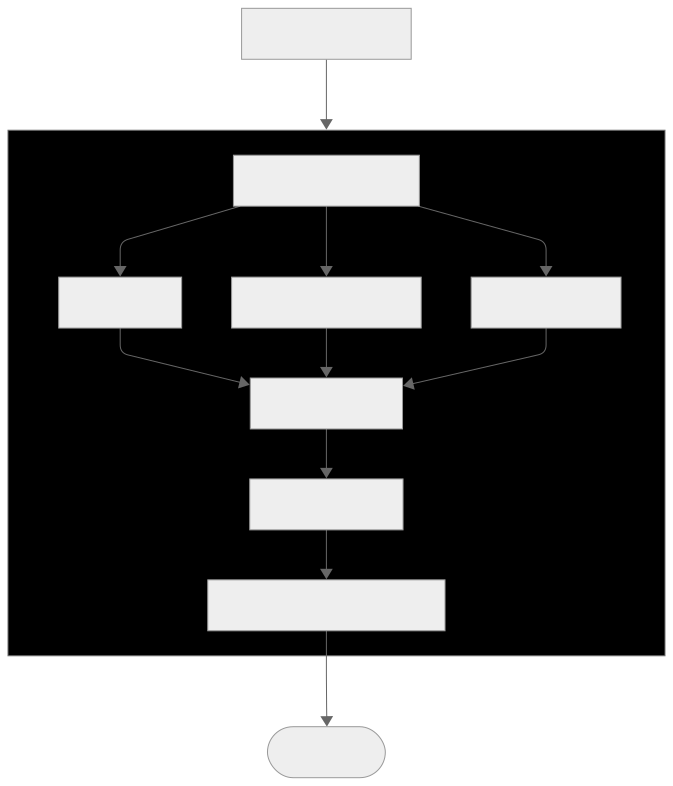
\includegraphics[width=\textwidth]{figures/loadingphase1.pdf}}
    \caption{The Loader Creation phase diagram}
    \label{fig:loadingphase1}
\end{figure}


Upon completion of the loader creation phase, a \texttt{Loader} object is produced that encapsulates the configuration 
template along with metadata about variables, constants, and execution parameters. 
\begin{minted}[fontsize=\footnotesize]{kotlin}
    interface Loader : Serializable {

    val constants: Map<String, Any?>
    val remoteDependencies: List<String>
    val launcher: Launcher
    val dependentVariables: Map<String, DependentVariable<*>>
    val variables: Map<String, Variable<*>>

    fun <T, P : Position<P>> getDefault(): Simulation<T, P>
    fun <T, P : Position<P>> getWith(values: Map<String, *>): Simulation<T, P>
    fun launch(launcher: Launcher = this.launcher): Unit
}
\end{minted}
\captionof{lstlisting}{Loader interface}

This loader serves as a factory for generating simulation instances. A Simulation can be generated by either
using the \textit{getDefault()} method, that will assign to each variable its default value, or by using the  
\textit{getWith()} method, that will assign to each variable the value provided in the map.

\paragraph{Simulation Instantiation Phase}
This phase occurs when \texttt{getDefault()} or \texttt{getWith()} is invoked with a map of variable values, that
represents the actual parameter values for that simulation instance.
So for each batch run, the getWith() method of the loader must be invoked.
This phase transforms the configuration template into an executable simulation model through the following steps:

\begin{itemize}
    \item \textbf{Variable reification}: Free variables receive their ground values from the provided map, 
    with defaults used for unspecified variables. The system validates that all provided variable names correspond 
    to known free variables.
    
    \item \textbf{Dependent variable computation}: Once all free variables have ground values, 
    dependent variables are evaluated using their registered computation functions. 
    The system ensures that all dependencies are satisfied before evaluation.
    
    \item \textbf{Simulation model construction}: The system constructs the complete simulation model, including:
    \begin{itemize}
        \item \textit{Incarnation} type of the simulation;
        \item \textit{Environment} instantiation with specified dimensions and properties;
        \item \textit{Nodes} creation and deployment according to deployment descriptors;
        \item \textit{Molecules} and concentration assignment to nodes;
        \item \textit{Reactions} and program attachment to nodes;
        \item \textit{Layers} configuration for spatial data structures;
        \item \textit{Linking rules} establishment for network topology;
        \item \textit{Monitors} and \textit{exporters} setup for data collection;
        \item \textit{Simulation engine} initialization
    \end{itemize}
In this phase, the system uses reflection\footnote{\url{http://archive.today/3rOQX}}
 combined with an automatic \textit{context parameter injection} mechanism
to support Alchemist's arbitrary class loading capabilities.

First, the system resolves the class name specified in the configuration by scanning the classpath, 
allowing users to refer to classes by their simple name if unambiguous.
Then, it instantiates the class using a dependency injection strategy:
the user provides only the parameters that define the specific configuration of the object,
while the system automatically injects contextual dependencies, such as the simulation environment, 
the random number generator, or the time distribution, if they are required by the selected constructor.
This is achieved by filtering out constructor parameters that match the types of available singletons in the loading context.
Consequently, these parameters do not need to be explicitly
defined in the configuration, reducing verbosity and decoupling the configuration from 
the internal wiring of the simulation components. 
\end{itemize}

\begin{figure}[H]
    \makebox[\textwidth][c]{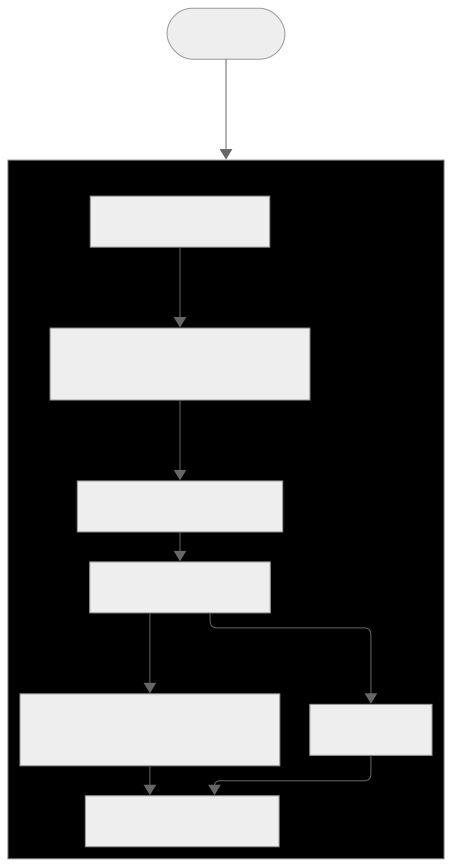
\includegraphics[width=0.4\textwidth]{figures/loadingphase2.pdf}}
    \caption{The Simulation Instantiation phase diagram}
    \label{fig:loadingphase2}
\end{figure}


This \textit{two-phase} loading system architecture provides several advantages:
\begin{enumerate}
    \item \textbf{Efficient batch execution}: a single loader can generate multiple simulation instances with different parameter
    combinations without re-parsing the configuration. 
    \item \textbf{Parameter space exploration}: by using custom launchers, the user can systematically vary 
    free variables across simulation runs.
    \item \textbf{Maintainability and extensibility}: the separation of concerns between configuration management 
    and simulation construction improves maintainability and extensibility.
\end{enumerate}

\subsection{Legacy Type System Limitations}

The Alchemist simulation model was designed to be generic over two fundamental types that define the nature of the simulated system:
\begin{itemize}
    \item \textbf{T (Concentration Type)}: Represents the type of data stored inside the nodes (molecules' concentration).
     This is defined by the specific \textit{Incarnation} used (e.g., \texttt{Double} for chemical simulations, 
     \texttt{Any} for aggregate computing).
    \item \textbf{P (Position Type)}: Represents the type of spatial coordinates used in the environment.
     This type must extend the \texttt{Position<P>} interface (e.g., \texttt{Euclidean2DPosition}, \texttt{GeoPosition}).
\end{itemize}

A fully type-safe simulation definition should theoretically propagate these two types, \texttt{<$T, P$>}, 
across all components: the \texttt{Environment}, \texttt{Nodes}, \texttt{Reactions}, and \texttt{Deployments} 
should all be parameterized consistently with the simulation's incarnation.
However, the legacy codebase presents some limitations in how these generics are handled,
 creating impedance mismatches for a statically typed DSL.

\subsubsection{Generic Type Erasure in Components}
Many existing Alchemist components were not designed with full generic propagation in mind. 
The crucial limitation lies in the class definitions themselves: rather than being generic classes that propagate the \texttt{T} and \texttt{P} types (e.g., \texttt{class Grid<P> : Deployment<P>}),
 many legacy components are non-generic and implement interfaces with \textbf{star-projections} (e.g., \texttt{Deployment<Position<*>>}).
This effectively erases the connection between the component and the specific types used in the simulation.

For instance, the \texttt{Grid} deployment class implements a star-projected interface: 

\begin{minted}[fontsize=\footnotesize]{kotlin}
open class Grid
constructor(
    private val environment: Environment<*, *>,
    private val randomGenerator: RandomGenerator,
    ... // other parameters
) : Deployment<Position<*>> 
\end{minted}

Passing a specific \texttt{Environment<T, P>} to this constructor is allowed because \texttt{Environment} is covariant (or the wildcard \texttt{<*, *>} accepts any projection).
The fundamental issue arises from the interface implemented by the class: \texttt{Deployment<Position<*>>}.
A type-safe DSL for a simulation with position type \texttt{P} requires Deployments of type \texttt{Deployment<P>}.
However, \texttt{Deployment<Position<*>>} is not a subtype of \texttt{Deployment<P>}.
Even if the \texttt{Grid} instance actually generates positions compatible with \texttt{P} (because it was initialized with an environment of type \texttt{P}), 
the type system cannot verify this relationship statically due to the erased type in the return interface.

To provide a seamless user experience, the DSL must bridge this gap. 
It should prevent the user from having to perform manual casts in their configuration scripts.
Consequently, the DSL implementation acts as an adapter layer that internally handles these type mismatches, often necessitating \textbf{unchecked casts} at runtime. 
This design choice explicitly sacrifices strict compile-time safety at the internal boundary to preserve the usability of the public API.

\subsubsection{The Loader Interface Limitation}
A similar limitation exists within the \texttt{Loader} interface itself. 
As shown in the analysis of the loading system, the \texttt{Loader} interface is not generic:

\begin{minted}[fontsize=\footnotesize]{kotlin}
interface Loader : Serializable {
    // ...
    fun <T, P : Position<P>> getWith(values: Map<String, *>): Simulation<T, P>
}
\end{minted}

The \texttt{Loader} object holds the simulation template (variables, deployments, etc.) but does not carry the \texttt{<T, P>}
 type information at the class level. 
The types $T, P$ are only introduced when the \texttt{getWith} method is invoked to instantiate the simulation, 
but there is no guarantee that the method types $T, P$ are the same as the types $T, P$ of the Simulation Object.
This implies that the internal representation of the simulation components within the \texttt{Loader} effectively
erases or hides their specific generic types.
Calling the \texttt{getWith()} method with different types $T, P$ will not result in different simulation models, since
the types are determined by the internal \texttt{Incarnation}. 
If the \texttt{getWith()} invocation method types $T_1, P_1$ are different from the actual simulation types $T_2, P_2$, the runtime cast will fail.

When the DSL constructs a \texttt{Loader}, it may have compile-time knowledge of $T, P$, 
but it must package this information into a non-generic \texttt{Loader} container, losing the type information.
Later, when \texttt{getWith} is called, the system must cast a \texttt{Simulation<T, P>} from these loosely typed components.

\section{Simulation Configuration Domain}
\label{sec:domain-model}

To design a type-safe DSL that effectively replaces the YAML configuration, it is necessary to formalize the domain model of an Alchemist simulation configuration. 
While the Alchemist core meta-model (described in Chapter~\ref{sec:background}) defines the runtime entities of a simulation, the \textbf{configuration domain} focuses on the declarative structures
 required to instantiate those entities.
This domain model identifies the key concepts, their properties, and the relationships that the DSL must express.

A simulation configuration in Alchemist is not merely a description of a single system state, but rather a \textbf{template} for generating one or more simulation instances.
The domain model is composed of three distinct areas of concern:
\begin{itemize}
    \item \textbf{Variables Definition}
    \item \textbf{Execution Settings}
    \item \textbf{Model Definition}
\end{itemize}

\subsection{Variables Definition}

Alchemist supports batch execution, allowing users to define a single configuration file that produces multiple simulation runs by varying parameters.
To support this, the configuration domain distinguishes between three types of values:
\begin{itemize}
    \item \textbf{Constants}: Values that remain fixed across all batch runs.
    \item \textbf{Free Variables}: Parameters that define the design space of the experiment. 
    They do not have a single value but a range or set of values. 
    The system generates a separate simulation for each combination of free variables.
    \item \textbf{Dependent Variables}: Values computed dynamically based on the current values of free variables (using formulas).
\end{itemize}
The DSL must provide mechanisms to declare these variables and use them transparently within the configuration, 
ensuring that type safety is maintained even when values are not known until runtime.

\subsection{Execution Settings}
\label{sec:execution-settings}
This part of the domain model configures \textit{how} the simulation is executed and observed, rather than \textit{what} is simulated.
It includes:
\begin{itemize}
    \item \textbf{Launcher}: The component responsible for managing the simulation lifecycle (such as batch mode or single run mode).
    \item \textbf{Seeds}: Configuration for the pseudo-random number generators. Alchemist typically separates the \textit{scenario RNG} (used for node placement) 
    from the \textit{simulation RNG} (used for stochastic events during execution) to ensure reproducibility.
    \item \textbf{Monitors}: Observers that track the simulation progress or status (e.g., logging to console, updating a GUI).
    \item \textbf{Exporters}: Specialized components responsible for data collection. 
    They export simulation data (e.g., molecule concentrations, node positions) to external formats (e.g., CSV, databases) for further analysis.
\end{itemize}

\subsection{Model Definition}

The Model Definition describes the actual system to be simulated. 
Key entities include:

\begin{itemize}
    \item \textbf{Incarnation}: The foundational factory that defines the type system for the simulation ($T, P$). All other components must be compatible with the types defined here.
    
    \item \textbf{Environment}: Represents the spatial context of the simulation (e.g., continuous 2D space, graph, grid). It dictates the Position type \texttt{P}.
    
    \item \textbf{Network Model}: Defines the topology of connections between nodes (e.g., nodes connected if within a certain distance). This is governed by \texttt{LinkingRules}.
    
    \item \textbf{Deployments}: Declarative generators that map geometric shapes (e.g., \texttt{Grid}, \texttt{Circle}) or algorithms to spatial positions. 
    They determine where nodes are initially placed in the environment.
    
    \item \textbf{Node Templates}: Define the internal structure of nodes. Since nodes are rarely configured individually, templates describe the properties of a generic node in a deployment:
    \begin{itemize}
        \item \textbf{Contents}: Initial \texttt{Molecules} and their \texttt{Concentrations}.
        \item \textbf{Programs}: The behavioral logic, composed of \texttt{Reactions}, which in turn consist of \texttt{Conditions}, \texttt{Actions}, and a \texttt{TimeDistribution}.
    \end{itemize}
    \item \textbf{Global Programs}: Logic that operates on the entire environment rather than being attached to specific nodes. 
    Similar to node programs, they are composed of \texttt{Global Reactions} that can modify the environment.
    \item \textbf{Layers}: Scalar fields mapped over the environment (e.g., to represent temperature or pollutant distribution) that nodes can sense.
\end{itemize}

%----------------------------------------------------------------------------------------
\chapter{Design}
\label{chap:design}
%----------------------------------------------------------------------------------------

This chapter details the architectural design of the proposed solution. 
The design follows a layered approach aimed at bridging the gap between the static, type-safe nature of the Kotlin language 
and the dynamic, reflection-based core of the Alchemist simulator.
The primary objective is to ensure full semantic equivalence with the existing configuration 
system while providing the benefits of a modern development environment.

\section{Architecture}

The architectural strategy exploits the capabilities of Kotlin as a General-Purpose Language (GPL)
 to achieve seamless integration with the existing Alchemist ecosystem.
The main design decision made is to grant users direct access to the underlying Alchemist codebase. 
In the legacy YAML configuration system, components are specified via their class names as strings, 
requiring a complex reflection-based mechanism to resolve and instantiate them at runtime.
Conversely, the proposed DSL allows users to instantiate these classes directly using standard Kotlin syntax, 
leveraging the fact that Alchemist components are native Java or Kotlin objects.

This approach eliminates the need for reflective class loading, shifting the responsibility 
of object instantiation from the framework to the language itself.
For instance, instantiating a \textit{network model} component becomes a direct constructor call:

\begin{minted}[fontsize=\footnotesize, linenos]{kotlin}
val networkModel = ConnectWithinDistance(0.5)
\end{minted}

In contrast, the YAML equivalent requires an indirect specification:
\begin{minted}[fontsize=\footnotesize, linenos]{yaml}
network-model:
  type: ConnectWithinDistance
  parameters: [0.5]
\end{minted}

By exposing the underlying API directly, the DSL inherits the type safety and tooling support of the host language. 
Users are compelled by the compiler to provide correct argument types and counts,
 transforming what were previously runtime configuration errors into compile-time checks.
Furthermore, this design ensures immediate compatibility with any future extensions to the Alchemist core,
 as any new class on the \textit{classpath} is automatically available for use within the DSL 
 without requiring updates to the parser logic.
 
Given this design decision, the next sections will detail how the new system should
 integrate with the existing loading system of Alchemist, 
and will describe the design decision made for the DSL itself.

\subsection{Loading System Integration}

To integrate with the existing Alchemist loading system, 
the proposed architecture introduces a new implementation of the \textbf{Loader} interface. 
As established in Section \ref{sec:loadingphase1}, the \textit{Loader} serves as a factory for simulation instances, 
parameterized by a set of variables that must be used in that specific simulation instance. 
The core mechanism relies on the method:
\begin{minted}[fontsize=\footnotesize, linenos]{kotlin}
fun <T, P : Position<P>> getWith(values: Map<String, *>): Simulation<T, P>
\end{minted}
\textbf{}
It \textbf{instantiates} a simulation by mapping variable names to the given set of specific values. 
This design decouples the generation of the simulation model from the management of configuration variables, 
allowing a single \textit{Loader} to generate multiple simulation instances with distinct parameter sets, 
an important enabler for batch execution.

The execution lifecycle is, instead, managed by the \textbf{Launcher} interface,
which accepts a \textit{Loader} as a dependency. 
The \textit{Launcher} is responsible for identifying the \textbf{variable space} (e.g., iterating over a set of parameters) 
and invoking the \textit{Loader} \texttt{getWith(values: Map<String, \*>)} method to create 
the corresponding simulation instances. 

\begin{figure}[H]
    \centering
    \includesvg[width=\textwidth]{figures/launcherloader}
    \caption{Loading system architecture}
    \label{fig:launcherLoader}
\end{figure}

As shown in the figure \ref{fig:launcherLoader}, the relationship between these components exhibits a bidirectional binding:
\begin{itemize}
    \item The \textit{Launcher} depends on the \textit{Loader} to obtain the simulation instance 
    (via the \texttt{getWith(values: Map<String, *>)} method).
    \item The \textit{Loader} holds a reference to the specified \textit{Launcher}, since the loader is the component 
    that holds all the needed information to generate a simulation given the user configuration. The \textit{Launcher} is a 
    configurable component that can be specified by the user to control the execution of the simulation
\end{itemize}


The loader component is the one that should be actually used to launch the simulation, using its 
\textit{launch} method:

\begin{minted}[fontsize=\footnotesize, linenos]{kotlin}
interface Loader {
    // ...
    fun launch(launcher: Launcher = this.launcher): Unit = launcher.launch(this)
}
\end{minted}

By adhering to this established contract, 
the new DSL-based implementation achieves full interoperability with the existing ecosystem. 
It acts as an alternative for the legacy loader, 
allowing existing \textit{Launcher} implementations to use the new DSL-based loader transparently 
via the \textit{Inversion of Control} (IoC) pattern.
Consequently, the complexity of the loading mechanism remains hidden from the user,
who retains the flexibility to specify custom \textit{Lauchers} without coupling the loader instance 
to a specific underlying \textit{Loader} implementation.


\subsection{Scoped Information Contexts}

To maintain the same semantic as the YAML configuration file and enforce domain rules, 
the architecture employs a \textit{Scoped Information Context} pattern. 
The simulation configuration is modeled not as a flat list of properties, but as a 
hierarchy of \textbf{nested contexts}, 
mirroring the structural containment of the domain entities.

In this model, the availability of operations and data is strictly determined by the current scope. 
For instance, the definition of a reaction makes sense only within the context of a node or a global program.
This design should somehow mimic the nesting levels in the YAML configuration file, but in a more \textit{type-safe} way.
While the YAML file allows, for example, to define a \textit{Deployment} inside a \textit{Deployment}, the nested context 
prevents the user to define such a configuration, since at each context level, only the allowed operations and data are available.
The relationship between the components, as shown in the figure \ref{fig:scoped-contexts}, is the following:

\begin{itemize}
    \item The \textbf{Simulation Context} is the root context, it contains all the execution settings, 
    as described in Section \ref{sec:execution-settings}. 
    \begin{itemize}
        \item Available elements: \textit{incarnation}, \textit{environment}, \textit{networkModel}, \textit{launcher}, \textit{simulationGenerator}, \textit{scenarioGenerator};
        \item Available operations: \textit{deployments}, \textit{programs}, \textit{monitors}, \textit{terminators}, \textit{exporter},
        \textit{layer}, \textit{variable}
    \end{itemize}

    \item The \textbf{Deployments Context} handles the creation of node deployments.
    \begin{itemize}
        \item Available elements: \textit{generator};
        \item Available operations: \textit{deploy}
    \end{itemize}

    \item The \textbf{Deployment Context} configures a specific deployment instance.
    \begin{itemize}
        \item Available elements: -;
        \item Available operations: \textit{all}, \textit{inside}, \textit{programs}, \textit{nodes}, \textit{properties}
    \end{itemize}

    \item The \textbf{Content Context} defines the molecules and concentrations for nodes.
    \begin{itemize}
        \item Available elements: \textit{filter}, \textit{molecule}, \textit{concentration};
        \item Available operations: -
    \end{itemize}

    \item The \textbf{Programs Context} manages the reaction programs for nodes.
    \begin{itemize}
        \item Available elements: -;
        \item Available operations: \textit{all}, \textit{inside}
    \end{itemize}

    \item The \textbf{Program Context} specifies the details of a reaction.
    \begin{itemize}
        \item Available elements: \textit{node}, \textit{program}, \textit{timeDistribution}, \textit{reaction};
        \item Available operations: \textit{timeDistribution}, \textit{addAction}, \textit{addCondition}
    \end{itemize}

    \item The \textbf{Properties Context} manages node properties.
    \begin{itemize}
        \item Available elements: -;
        \item Available operations: \textit{all}, \textit{inside}
    \end{itemize}

    \item The \textbf{Property Context} assigns properties to nodes.
    \begin{itemize}
        \item Available elements: \textit{filter}, \textit{node};
        \item Available operations: \textit{add}
    \end{itemize}

    \item The \textbf{Exporter Context} configures data export.
    \begin{itemize}
        \item Available elements: \textit{type};
        \item Available operations: \textit{data}
    \end{itemize}

    \item The \textbf{Layer Context} defines spatial layers.
    \begin{itemize}
        \item Available elements: \textit{molecule}, \textit{layer};
        \item Available operations: -
    \end{itemize}

    \item The \textbf{Terminators Context}, \textit{Output Monitors Context}, and \textit{Global Programs Context} allow adding respective components.
    \begin{itemize}
        \item Available elements: -;
        \item Available operations: \textit{add} 
    \end{itemize}
\end{itemize}

This hierarchical design has been extracted from the Alchemist YAML specification, 
and it is a direct translation of the YAML hierarchy into the DSL, with some minor syntax 
changes.

\begin{figure}[H]
    \centering
    \includesvg[width=\textwidth]{figures/contexts}
    \caption{Scoped Information Contexts diagram}\label{fig:scoped-contexts}
\end{figure}

This hierarchical design serves two purposes:
\begin{enumerate}
    \item \textbf{Scope Containment}: It prevents structural inconsistencies by restricting the visibility of methods.
     A user cannot accidentally define a deployment inside a deployment because the \textit{Deployment Context} 
     does not expose the API for deployments creation.
    \item \textbf{Context Awareness}: Inner scopes transparently inherit relevant information from outer scopes. 
    A node definition context automatically has access to the environment type defined in the parent scope, 
    eliminating the need for redundant type specifications.
\end{enumerate}

\section{Detailed Design}

This section delves into the internal mechanisms 
that enable the DSL to function as a configuration template for multiple simulation runs.

\subsection{Deferred Execution Model}

A critical requirement for the Alchemist simulator is the support for \textit{batch executions}, 
where a single configuration file generates multiple simulation instances with varying parameters. 
A naive implementation of the DSL might instantiate the simulation objects immediately during script execution. 
However, this would bind the simulation to a single set of values, breaking the batching requirement.

To address this, the design adopts a \textbf{Lazy Evaluation} model, essentially a variation of the 
\textit{Command Pattern}\footnote{\url{https://archive.is/vwOm2}}. 
When the DSL script is executed, it does not construct the simulation entities (nodes, deployments, reactions) directly. 
Instead, it records a sequence of "build tasks" or specifications. This already happens in the current YAML loader, 
where the simulation model is actually built only when the \texttt{getWith()} method,  of the loader, is invoked.


The process is divided into two distinct phases:
\begin{enumerate}
    \item \textbf{Definition Phase}: The script runs once. 
    It builds an internal representation of the user's intent, a recipe for how to build the simulation. 
    Each DSL operation is stored as a \textbf{build step}, that will be later executed to modify the simulation model.
    During this phase, variables are treated as symbolic references rather than concrete values. In this phase, the 
    variables must not be accessed, since they are not yet assigned any value. This phase should produce 
    an \textbf{SimulationContext} instance that stores all the needed information to 
    later allow the DSL loader component to materialize the simulation model, 
    given the variable values for the current run. This \textit{SimulationContext} instance should be considered as the \textit{recipe}
    of the simulation, that will later be used to materialize the simulation model.
    \item \textbf{Materialization Phase}: This occurs repeatedly, once for each simulation in a batch. 
    The \textit{DSL Loader} invokes the recorded build tasks of the given \textit{SimulationContext} instance 
    after injecting the specific variable values (the \textit{grounding}) 
    for the current run.
\end{enumerate}

\begin{figure}[H]
    \centering
    \includesvg[width=0.5\textwidth]{figures/lazyeval}
    \caption{Lazy Evaluation model diagram}\label{fig:lazyeval}
\end{figure}


Since the user should be able to reference variables in the DSL, the lazy evaluation design prevents
the DSL execution to access variables values that are not yet assigned by the launcher. Suppose the DSL 
script is directly executed during its evaluation phase, the variables would be accessed before they are assigned
any values. Moreover, directly executing the DSL script would require to re-execute 
the script for each simulation in the batch. 


This separation of concerns ensures that the computational overhead of evaluating the script is paid only once,
 while the lightweight \textit{materialization phase} can be repeated efficiently for a batch of independent runs.

\subsection{Variables Management}

One of the primary challenges in adapting a General-Purpose Language for simulation configuration is the handling
of variable state across batch executions.
In a standard imperative program, variable assignment is immediate and bound to the current execution scope.
However, the Alchemist batch execution model requires the same configuration logic to be re-evaluated against 
a changing set of parameters. 
If variables were resolved at the time of script definition, 
the simulation would be bound to a single static configuration, negating the purpose of the batch mechanism.

To address this, the proposed design abstracts the concept of a variable from a direct value holder 
to a \textbf{reference} to a certain value in a \textbf{variables' registry}. 
Leveraging the semantic capabilities of the host language, 
variables defined in the DSL do not store data directly. 
Instead, they function as keys that query a centralized \textit{Variables Context}, a scoped container responsible
for managing the state of the simulation parameters.

Under this paradigm, the declaration of a variable registers the identifier within
 the context but defers value resolution. 
 The actual binding of values occurs solely during the \textit{materialization phase} described in the previous section. 
 When the \textit{Loader} prepares a specific simulation instance, 
 it populates the \textit{Variables Context} with the distinct combination of parameters assigned to that run.
Consequently, when the DSL logic subsequently accesses the variable, the request is fetched from the \textit{Variables Context}.

This architecture effectively decouples the definition of the simulation structure from the data that drives it.
It ensures that the same compilation of the DSL script can support an arbitrary number of execution instances,
 each perceiving a unique, consistent view of the variable space. 
Figure \ref{fig:variable-proxy} shows this interaction.

\begin{figure}[H]
    \centering
    \includesvg[width=0.4\textwidth]{figures/variablesdesign}
    \caption{Variables Context design diagram}
    \label{fig:variable-proxy}
\end{figure}

The low-level details of this mechanism,
particularly the integration with Kotlin language features, are provided in the Implementation chapter.

%----------------------------------------------------------------------------------------
\chapter{Implementation}
\label{chap:implementation}
%----------------------------------------------------------------------------------------

\section{DSL Implementation} %TODO: Stepped incremenetal implmenetations
\subsection{DSL Builder Functions}
\subsection{Variables and Constants}
\subsection{Integration with Existing Loading System}
\section{KSP Implementation}
\subsection{Symbol Processing Pipeline}
\subsection{Code Generation Strategy}
\subsection{Context Injection Mechanism}




%----------------------------------------------------------------------------------------
\chapter{Evaluation}
\label{chap:evaluation}
%----------------------------------------------------------------------------------------

The evaluation of the Alchemist DSL focuses on verifying that the solution meets 
the functional and non-functional requirements outlined in \Cref{chap:analysis}. 
The assessment is divided into two main parts: 
a technical validation through two different testing strategies,
 and a qualitative discussion on the benefits introduced by the new system.

\section{Testing Strategy}
\label{sec:testing}

The testing process was designed to ensure correctness, equivalence with the legacy system, and performance stability. 
The strategy followed an incremental approach, starting from the unit testing of individual DSL components,
 proceeding to the structural validation of the generated simulation models, 
 and concluding with runtime behavior comparison and performance testing.

\subsection{Unit Testing}
\label{subsec:unit-testing}

The unit testing phase focused on validating the core architectural mechanisms of the DSL rather than exhaustively 
covering every possible configuration option. 
Given that the DSL relies on a consistent recursive builder pattern, the strategy prioritized the verification of 
the most complex and critical infrastructure components: the variable management system and the 
type-safe context propagation.

The \textbf{Variables Context} received the most extensive unit testing coverage due to its central 
role in enabling batch executions. 
Unit tests specifically targeted this component to ensure that the delegation mechanism correctly captures default 
values during the definition phase and that the \texttt{DSLLoader} successfully injects run-specific values
 during the materialization phase. 
This isolation ensured that the complex logic handling dependent variables and potential circular dependencies was
 robust before being integrated into the full simulation loader.

Beyond variables, unit tests were employed to validate the fundamental building blocks of the DSL structure,
 such as the root \texttt{SimulationContext} and the primary nested contexts like \texttt{Deployments Context}.
The primary objective was to verify the correct propagation of the generic types $T$ (concentration) and $P$ (position)
 throughout the context hierarchy. 
These tests confirmed that the Kotlin compiler and the DSL infrastructure correctly enforced type constraints,
 preventing type mismatches within nested blocks.

However, an exhaustive unit test for every specific domain entity (e.g., every available reaction, condition, or deployment type)
 was deemed redundant at this stage. 
Since the DSL leverages a uniform builder pattern, once the core mechanisms, such as context nesting, property delegation, 
and builder execution, were validated on the main components, the correctness of the broader domain coverage was
 delegated to the \textbf{Equivalence Testing} phase. 
This strategy avoided determining the correctness of individual wrappers, 
relying instead on the comprehensive verification against the legacy YAML system to catch any discrepancies in the generated models.

\subsubsection{Processor Verification}

In addition, the Kotlin Symbol Processing (KSP) component (described in \Cref{sec:ksp-implementation}) 
required a dedicated testing strategy. 
Since the processor is responsible for generating the bridge code that makes the DSL more user-friendly,
 its correctness is a key factor for the user experience.

The unit testing for the processor involved the compilation of synthetic Kotlin sources annotated with \texttt{@AlchemistKotlinDSL}. 
The tests asserted that the processor:
\begin{itemize}
    \item Correctly identified the primary constructors of annotated classes.
    \item Accurately distinguished between user-configurable parameters and system-injectable
     dependencies (e.g., \texttt{Environment}, \texttt{RandomGenerator}, etc.).
    \item Generated factory functions with the correct signature, including appropriate context receivers and generic constraints.
    \item Correctly synthesized the accessor paths (e.g., mapping a request for `Environment` to the correct parent context property)
     to solve the context chaining problem.
\end{itemize}

\subsection{Equivalence Testing}
\label{subsec:equivalence-testing}

To demonstrate compliance with the \textbf{YAML equivalence} requirement, an integration test suite was developed. 
The objective was to prove that for any valid YAML configuration, a semantically \textbf{identical} DSL script exists and produces 
an indistinguishable simulation model.
This verification relies on a set of \textit{reference scenarios}, covering the full spectrum of Alchemist features, 
from simple node placement to complex environment-aware movement and reaction programs.
This type of test is the core tool to verify the correctness of the DSL. It \textbf{must} be used to 
ensure that the DSL is able to produce the same simulation model as the YAML loader. 
The strategy used to test the DSL was to adopt a bottom-up approach, starting from the simplest scenarios 
and gradually adding complexity. This approach allowed identifying and fixing issues early on, 
giving a clear path to the final solution.

The validation process utilizes a custom comparison framework, which performs verification at two levels:
\begin{itemize}
    \item \textbf{Static Structural Comparison}: verifies that the DSL produces a simulation model 
    identical to the YAML loader's output before execution begins.
    \item \textbf{Runtime Behavioral Comparison}: run the simulation for a certain number of steps or until a certain time,
    and then compare the final state of the simulation.
\end{itemize}

\subsubsection{Static Structural Comparison}

The \texttt{StaticComparisonHelper} verifies that the DSL produces a simulation 
model identical to the YAML loader's output before execution begins. 
It inspects the \texttt{Loader} objects produced by both systems and compares the resulting simulation instances deeply.
Key verification points include:
\begin{itemize}
    \item \textbf{Variable Metadata}: asserting that the set of declared variables and their default values are identical.
    \item \textbf{Environment Configuration}: checking that node counts and positions match.
    \item \textbf{Node State}: verifying that every node is initialized at the exact same
    coordinates and contains the same set of molecules and concentrations.
    \item \textbf{Program Structure}: inspecting the reactions attached to nodes to ensure they have the same conditions,
     actions, and time distributions.
\end{itemize}
This phase ensures that the DSL syntax correctly maps to the underlying domain model structure.
However, this static analysis approach encountered significant limitations due to the legacy nature of the Alchemist codebase. 
Many core interfaces and classes do not expose their full internal state or do not implement value-based \texttt{equals()} methods, 
relying instead on reference equality. 
Verifying that two distinct instances of a complex object (e.g., a \texttt{TimeDistribution} or a \texttt{Layer}) are semantically 
identical proved difficult without resorting to fragile reflection-based inspection of private fields. 

To mitigate this, the static comparison often relies on proxy indicators, such as verifying that the class types 
match (via class name inspection) or comparing the string representation (\texttt{toString()}) of components. 
While useful for catching gross configuration errors, 
these checks cannot guarantee that two objects have identical internal configurations if their string representations are incomplete.

\subsubsection{Runtime Behavioral Comparison}

To overcome the limitations of static inspection and guarantee true semantic equivalence,
the evaluation strategy introduced a \textbf{Runtime Behavioral Comparison}. 
The rationale is that if two simulations are configured identically, 
and the underlying simulator is deterministic (given the same random seed), 
they must evolve through identical states over time.

The \texttt{RuntimeComparisonHelper} executes both the YAML-generated and DSL-generated simulations,
 stepping them forward for a fixed duration or a specific number of steps. 
At the end of this execution, the framework compares the tangible, observable state of the simulation—properties that are 
publicly accessible and critical to the simulation's outcome:
\begin{itemize}
    \item \textbf{Global State}: Asserting that both simulations reached the exact same simulation time and step count.
    \item \textbf{Node Positions}: Verifying that the coordinates of every node match, 
    confirming that movement logic and environment boundaries are the same.
    \item \textbf{Node Contents}: Checking that the set of molecules and their concentrations inside each node are identical,
     confirming that reactions and diffusion processes executed in the same order and with the same effects.
\end{itemize}
This dynamic verification provides a much stronger guarantee of correctness than static analysis. 
It confirms not only that the components are of the right type, but that they were initialized with
 the correct parameters and that the Random Number Generators (RNGs) were consumed in the exact same 
 sequence, a crucial factor for reproducibility in stochastic simulations.

\subsection{Performance Testing}
\label{subsec:performance-testing}

While the primary goal of the DSL is usability and safety, the \textbf{performance} of the loading phase must 
remain within acceptable limits. 
The \texttt{PerformanceComparisonTest} suite benchmarks the initialization time of the DSL against the YAML loader.
The tests measure the time required to parse the configuration and produce a ready-to-run \texttt{Simulation} object.
While the YAML loader is slightly faster than the DSL in raw loading speed, due to the overhead of Kotlin script compilation
and class loading, the tests aim to verify that the overhead remains acceptable.
The results show that while there is a distinct initial \textit{warm-up} cost for the Kotlin script engine,
the impact on the overall workflow is mitigated by the batch execution model, 
where the script is compiled only once for an arbitrary number of simulation runs.
The tests verify that the overhead remains acceptable and that the DSL is not significantly slower than the YAML loader.
The test was made using a moderately complex simulation configuration, as shown in \Cref{lst:complextestsim}.



\begin{center}
    \begin{minipage}{0.48\textwidth}
    \inputminted[
      fontsize=\tiny,
      breaklines,
      firstline=1,
      lastline=42, 
      linenos
    ]{kotlin}{listings/complextestsim.kts}
    \end{minipage}
    \hfill
    \begin{minipage}{0.48\textwidth}
    \inputminted[
      fontsize=\tiny,
      breaklines,
      firstline=43,
      lastline=80, 
      linenos
    ]{kotlin}{listings/complextestsim.kts}
    \end{minipage}
    \captionof{lstlisting}
    {Simulation configuration used for the performance test}
    \label{lst:complextestsim}
\end{center}
\newpage
    



\Cref{tab:performance-results} presents the performance comparison results obtained 
from 20 iterations of both the loading phase, and the action phase separately.
The test measures the time required to load and initialize the simulation 
configuration using both the YAML loader and the DSL loader.


\begin{table}[h]
\centering
\caption{Performance comparison results (20 iterations)}
\label{tab:performance-results}
\begin{tabular}{l|r|r}
\textbf{Phase} & \textbf{YAML (ms)} & \textbf{DSL (ms)} \\
\hline
\textbf{Loading Phase} & 11,002 & 15,802 \\
\hline
\textbf{Action Phase} & 4,422 & 2,734 \\
\hline
\textbf{Total Average} & \textbf{15,424} & \textbf{18,536} \\
\end{tabular}
\end{table}

The results reveal an interesting performance profile: while the DSL is slower during the \textbf{Loading Phase}, 
it performs better than the YAML loader during the \textbf{Action Phase}.
This performance difference can be attributed to the fact that the Loading Phase includes the overhead of Kotlin script compilation, 
which is a one-time cost that occurs when the script is first processed.
However, once the configuration is loaded, the DSL's materialization process is more efficient, resulting in faster Action Phase execution.
The overall performance shows that YAML is approximately 20\% faster in total time, but this overhead is acceptable given the benefits in terms of type safety, 
IDE support, and code reusability.
Moreover, in batch execution scenarios where the script is compiled once and used for multiple simulation runs,
 the Loading Phase cost is amortized, making the DSL's superior Action Phase performance more significant.

\section{Experimental Evaluation}
\label{sec:experimental-evaluation}

Beyond technical correctness, the success of the DSL is measured by how well it fulfills the user-centric 
goals of usability, 
type safety, and expressiveness. 
This section evaluates the impact of the new system on the developer experience, 
comparing it qualitatively against the legacy YAML-based workflow.

\subsection{DSL Usability and Expressiveness}
\label{subsec:usability}

The adoption of Kotlin as the host language transforms the configuration process from writing passive data 
descriptions (YAML) 
to developing active simulation software. 
This shift introduces several key improvements in usability:

\begin{itemize}
    \item \textbf{IDE-Assisted Development}: Unlike YAML, where users must rely on external documentation or 
    schema validators (often incomplete), the DSL benefits from the full power of the IDE. 
    Features such as \textbf{auto-completion} allow users to explore the available API surface interactively. 
    For instance, typing \texttt{this.} instantly suggests all available properties and methods of the current context,
    drastically reducing the need to switch context to read the documentation.
    
    \item \textbf{Type Safety as Feedback}: The static type system acts as an immediate feedback loop. 
    Errors such as assigning a \texttt{Double} to an \texttt{Int} parameter, or attempting to use a 2D position in
     a generic implementation, are flagged at compile-time (or edit-time in the IDE) rather 
     than crashing the simulation at runtime. Furthermore, users can leverage standard Kotlin language constructs,
     such as \texttt{for} loops, \texttt{if} statements, and other control flow primitives, enabling more expressive and flexible
     simulation configurations.

    \item \textbf{Scope Safety}: The use of \texttt{@AlchemistDsl} annotations (as detailed in \Cref{chap:implementation}) 
    successfully solved the structural ambiguity problem. 
    The compiler now enforces the domain hierarchy, making it syntactically impossible to nest 
    components incorrectly (e.g., defining a node inside a reaction). 
    This provides a structural guarantee that the YAML parser could only approximate through runtime validation.
\end{itemize}

One of the most powerful advantages of using Kotlin as the host language is the ability to create reusable 
components and functions that can be shared across multiple simulation files. 
Unlike YAML, where configuration must be duplicated or manually copied between files, 
the DSL enables users to define common patterns as functions or extension functions, 
which can be imported and reused throughout their project. 
This approach promotes code reuse, reduces duplication, and ensures consistency across simulations.

Consider, for example, a scenario where multiple simulations require a similar deployment pattern, 
such as a grid-based node placement with a specific reaction configuration. 
In YAML, this pattern would need to be replicated in each configuration file, 
making it difficult to maintain consistency and apply changes uniformly. 

\begin{minted}[fontsize=\scriptsize, linenos]{YAML}
incarnation: sapere
environment: { type: OSMEnvironment }
network-model: { type: ConnectWithinDistance, parameters: [1000] }
_venice_lagoon: &lagoon
  [[45.2038121, 12.2504425], [45.2207426, 12.2641754], [45.2381516, 12.2806549],
   [45.2570053, 12.2895813], [45.276336, 12.2957611], [45.3029049, 12.2991943],
   [45.3212544, 12.3046875], [45.331875, 12.3040009], [45.3453893, 12.3040009],
   [45.3502151, 12.3156738], [45.3622776, 12.3232269], [45.3719259, 12.3300934],
   [45.3830193, 12.3348999], [45.395557, 12.3445129], [45.3998964, 12.3300934],
   [45.4018249, 12.3136139], [45.4105023, 12.3122406], [45.4167685, 12.311554],
   [45.4278531, 12.3012543], [45.4408627, 12.2902679], [45.4355628, 12.2772217],
   [45.4206242, 12.2703552], [45.3994143, 12.2744751], [45.3738553, 12.2676086],
   [45.3579354, 12.2614288], [45.3429763, 12.2497559], [45.3198059, 12.2408295],
   [45.2975921, 12.2346497], [45.2802014, 12.2408295], [45.257972, 12.233963],
   [45.2038121, 12.2504425]]
deployments:
  type: Polygon
  parameters: [500, *lagoon]
  programs:
    - time-distribution: 10
      type: Event
\end{minted}
\captionof{lstlisting}{Example of a YAML simulation script with a complex deployment}

With the Kotlin DSL, users can define a reusable function that encapsulates this pattern:

\begin{minted}[fontsize=\scriptsize, linenos]{kotlin}
fun createLagoon() = listOf(
    45.2038121 to 12.2504425, 45.2207426 to 12.2641754, 45.2381516 to 12.2806549,
    45.2570053 to 12.2895813, 45.276336 to 12.2957611, 45.3029049 to 12.2991943,
    45.3212544 to 12.3046875, 45.331875 to 12.3040009, 45.3453893 to 12.3040009,
    45.3502151 to 12.3156738, 45.3622776 to 12.3232269, 45.3719259 to 12.3300934,
    45.3830193 to 12.3348999, 45.395557 to 12.3445129, 45.3998964 to 12.3300934,
    45.4018249 to 12.3136139, 45.4105023 to 12.3122406, 45.4167685 to 12.311554,
    45.4278531 to 12.3012543, 45.4408627 to 12.2902679, 45.4355628 to 12.2772217,
    45.4206242 to 12.2703552, 45.3994143 to 12.2744751, 45.3738553 to 12.2676086,
    45.3579354 to 12.2614288, 45.3429763 to 12.2497559, 45.3198059 to 12.2408295,
    45.2975921 to 12.2346497, 45.2802014 to 12.2408295, 45.257972 to 12.233963,
    45.2038121 to 12.2504425,
)
\end{minted}
\captionof{lstlisting}{Example of a reusable deployment function}

The \textit{createLagoon} function can now be used to create a lagoon deployment in any simulation script:

\begin{minted}[fontsize=\footnotesize, linenos]{kotlin}
simulation(incarnation) {
    networkModel = ConnectWithinDistance(1000.0)
    deployments {
        val lagoon = createLagoon()
        deploy(polygon(500, lagoon)) {
            programs {
                all {
                    timeDistribution("10")
                    reaction = event()
                }
            }
        }
    }
}
\end{minted}

This approach makes the configuration more readable and maintainable. 
Modifying the lagoon deployment requires only updating the \textit{createLagoon} function, 
without the need to update all configurations that use it.

Another approach is to directly define new DSL blocks to match the simulation domain. 
For example, a \textit{lagoon} block can be defined as follows:

\begin{minted}[fontsize=\footnotesize, linenos]{kotlin}
simulation(incarnation) {
    networkModel = ConnectWithinDistance(1000.0)
    deployments {
        lagoon(500) {
            programs {
                all {
                    timeDistribution("10")
                    reaction = event()
                }
            }
        }
    }
}
\end{minted}

The key benefit of this approach is that users can customize the DSL to match their specific simulation 
domain by creating reusable libraries or modules. 
These domain-specific extensions can define functions and DSL blocks with names and structures 
that align with the terminology and concepts of the target domain, 
such as \texttt{lagoon}, \texttt{swarm}, or \texttt{agent}. 
This domain-driven customization significantly enhances the readability of simulation scripts, 
as the syntax becomes more intuitive and self-documenting for domain experts. 
Furthermore, it provides users with greater control over the DSL syntax, 
enabling them to create abstractions that precisely match their modeling needs 
while maintaining full type safety and IDE support.

Finally, users can leverage standard Kotlin language features to create more complex simulations. 
For example, they can use \texttt{for} loops or \texttt{if} statements to create more complex situations 
without manually listing all possible cases.
\begin{minted}[fontsize=\footnotesize, linenos]{kotlin}
simulation(incarnation, { env }) {
    deployments {
        for (i in 1..10) {
            for (j in 1..10) {
                if (i == j) continue
                deploy(point(i.toDouble(), j.toDouble())){
                    // ...
                }
            }
        }
    }
}
\end{minted}

This example demonstrates only a simple usage of standard Kotlin language features to create more complex simulations. 
However, this design allows users to fully customize the DSL to match their specific simulation domain.

\subsection{Impact of the KSP Processor}
\label{subsec:ksp-evaluation}

The introduction of the KSP processor was a \textbf{decisive} factor in making the DSL usable in practice. 
Without the automatic generation of bridge code, the DSL would have suffered from severe verbosity, 
requiring users to manually inject system dependencies (like \texttt{environment} or \texttt{randomGenerator}) into every component constructor.
In the example below (\Cref{lst:example-verbose}), the usage of a \textit{BrownianMove} reaction would have been very verbose, since the reaction 
block is deeply nested in the context hierarchy. In this case, the reaction also requires several internal parameters to be passed to the constructor, 
reducing the readability of the code.


\begin{minted}[fontsize=\footnotesize, linenos]{kotlin}
simulation(incarnation) {
    networkModel = ConnectWithinDistance(1000.0)
    deployments {
        lagoon(500) {
            programs {
                all {
                    timeDistribution("10")
                    reaction = Event(node, timeDistribution)
                    addAction {
                        BrownianMove(
                            env,
                            node,
                            ctx.ctx.ctx.ctx.simulationGenerator,
                            0.0005,
                        )
                    }
                }
            }
        }
    }
}
\end{minted}
\label{lst:example-verbose}
\captionof{lstlisting}{Example of a simulation script with no helper functions}

With the KSP processor, it generates a helper function that can be used to create the reaction (as shown in \Cref{lst:example-helper}), 
simplifying the code and improving the readability. It also avoids the need to manually inject the system dependencies into the constructor, 
since they are injected automatically by the helper function.
\newpage
\begin{minted}[fontsize=\footnotesize, linenos]{kotlin}
simulation(incarnation) {
    networkModel = ConnectWithinDistance(1000.0)
    deployments {
        lagoon(500) {
            programs {
                all {
                    timeDistribution("10")
                    reaction = event()
                    addAction {
                        brownianMove(0.0005)
                    }
                }
            }
        }
    }
}
\end{minted}
\label{lst:example-helper}
\captionof{lstlisting}{Example of simulation script with helper functions}

Note that, by default, the generated functions are defined using the same name of the object they are generating, 
but with the first letter in lowercase. This should simplify the usage of the helper functions, since users can just
use the lowercase version of the object name to call the helper function. 

%----------------------------------------------------------------------------------------
\chapter{Conclusion and Future Work}
\label{chap:conclusion}
%----------------------------------------------------------------------------------------

\paragraph{Conclusion}

This thesis presents a methodology for constructing type-safe internal Domain-Specific Languages that replace untyped 
declarative configuration formats with General-Purpose Language-based solutions, preserving semantic equivalence while 
introducing compile-time safety and enhanced developer experience.

The central insight of this work is that internal DSLs built on modern language features can successfully reconcile 
the static verification requirements of type-safe systems with the dynamic extensibility demands of complex frameworks. 
Rather than requiring extensive refactoring of existing codebases, the approach employs code generation techniques 
to bridge the gap between simplified DSL APIs and legacy component interfaces, enabling incremental adoption without 
compromising type safety or usability.

A key finding is that generative approaches, specifically leveraging compiler plugin APIs like Kotlin Symbol Processing, 
provide a practical pathway for integrating DSLs with systems that were not originally designed for type-safe configuration. 
This technique addresses the fundamental tension between static verification and runtime flexibility, offering a scalable 
solution applicable beyond the immediate use case.

The methodology demonstrates that transitioning from data-serialization formats to type-safe configuration languages 
yields substantial benefits: errors are caught during development rather than execution, tooling support becomes 
comprehensive rather than limited, and configuration evolves from monolithic files to composable, reusable modules. 
These advantages become particularly pronounced in domains with complex, recurring configuration patterns.

The Alchemist simulation framework serves as a concrete validation of this methodology, demonstrating its applicability 
to a real-world, extensible system. The resulting DSL maintains full semantic equivalence with the legacy YAML-based 
configuration while providing the type safety, tooling support, and modularity benefits that justify the transition 
from untyped to type-safe configuration languages.


\paragraph{Future Work}

While the current implementation successfully addresses the core requirements, several directions for future enhancement
present themselves.
A natural extension would be the development of conversion tools that enable seamless migration between YAML and DSL formats. 
A \textbf{YAML-to-DSL converter} could automatically translate existing YAML configurations into equivalent DSL scripts,
facilitating the migration of legacy configurations.

Currently, the DSL handles node programs as generic string values, 
requiring users to write reactions using the native syntax of each 
incarnation (e.g., \texttt{"\{token\} --> \{firing\}"}).
While this approach maintains compatibility with the existing Alchemist architecture, 
it sacrifices the type safety and IDE support that are core benefits of the DSL.

Future work could extend the DSL to support \textbf{custom} DSLs for each incarnation, allowing users to define 
programs using incarnation-specific syntax that is fully integrated with Kotlin's type system. 
For example, instead of string-based 
reaction definitions, the SAPERE incarnation could provide a DSL that allows users to define eco-laws using type-safe constructs:
\begin{minted}[fontsize=\footnotesize, linenos]{kotlin}
sapere {
    deployments {
        programs {
            ecoLaw {
                consume("token")
                produce("firing")
            }
        }
    }
}
\end{minted}



%----------------------------------------------------------------------------------------
% BIBLIOGRAPHY
%----------------------------------------------------------------------------------------

\backmatter

\nocite{*} % Remove this as soon as you have the first citation

\bibliographystyle{unsrt}
\bibliography{bibliography}

\begin{acknowledgements} % this is optional remember to add chicco
Optional. Max 1 page.
\end{acknowledgements}

\end{document}
